\ifthenelse{\boolean{pcppapermadweb}}{}{
\chapter{On Password Composition and Complexity}
\label{chp4::password-composition}

In this chapter, we empirically investigate the composition of passwords. Our aim is to understand why common passwords are weak and how we can strengthen them. The subsequent chapter will focus on how passwords are guessed. While numerous studies have provided high-level analyses of password structure and composition, we take this further by presenting the first human-labelled password dataset. We also address issues in the choice of Password Composition Policies (PCPs) and demonstrate how our dataset aids in creating stronger and more usable passwords---we recommend a five-word PCP.
}

\section{Introduction}

The lack of consensus on Password Composition Policies (PCPs) and the lack of adoption of best practices on the web~\cite{lee_password_2022} suggest that our knowledge of password security is not yet complete. Password Strength Meters (PSMs), such as the \zxcvbn PSM, which was found to be the best dictionary-based PSM by Wang~\etal~\cite{wang_no_2023} and has 14.7K GitHub stars, still have obvious weak points. For example, \zxcvbn gives the password \password{girlsruledaworld} a maximum score of 4 (scores range from 1 to 4). It also assigns a strong score of 3/4 to \password{asdf1fdsa1}. This is because PSMs such as \zxcvbn depend on the patterns and structures they are programmed to recognise. This raises the question of what other patterns we are missing. To advance our understanding of passwords, we provide the first human-labelled password dataset.

\begin{figure}[t]
    \centering
    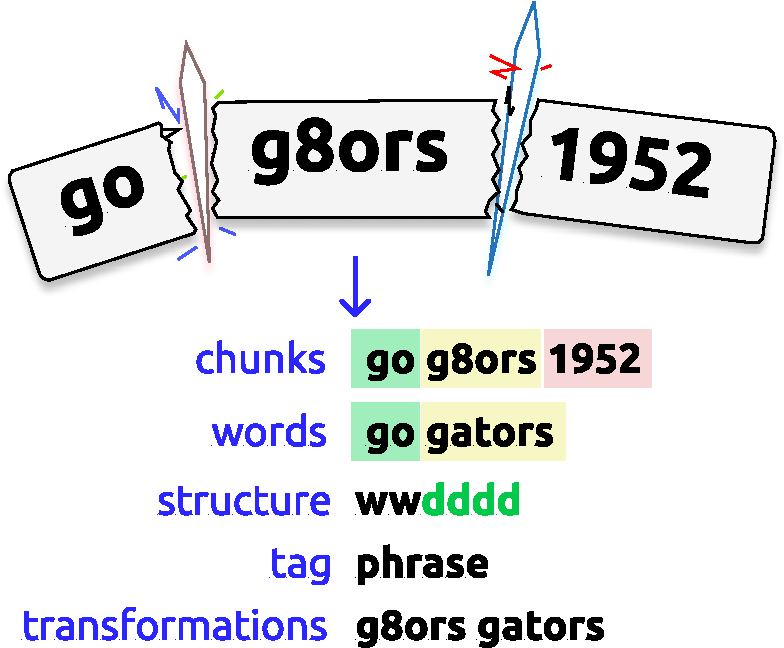
\includegraphics[scale=0.5]{figs/why_passwords/intro_fig.pdf}
    \caption{Example of the labelling process. The password \texttt{gog8ors1952} is sliced into core constituents, then the meaningful words are extracted. Such a labelling process can capture details such as transformations. \srcOwnFig}
    \label{fig:intro_password}
    %\vspace{-1em} % Adjust the negative value to reduce the gap
\end{figure}

It is almost common knowledge that we embed personal information in our secrets and that they possess a certain structure. But have we studied and collected most of these patterns and structures? The implications are important, as we saw with the \zxcvbn example---users can be misled into believing their secrets are strong enough. Other fields benefit from a plethora of labelled datasets that can be analysed; unfortunately, such a dataset does not exist in web security, specifically in password security. The chief task of this chapter is to human-label such a dataset and propose new methods to advance our understanding of password compositions.

We manually label the \hmail (2009) dataset~\cite{miessler_hotmail_2009} and machine-label the Lizard Squad dataset (2015)~\cite{miessler_lizardsquad_2015}. We are also in the process of fully labelling the Fortinet (2022) dataset~\cite{miessler_fortinet_2021}. The dataset itself is the key contribution of this chapter, and we discuss many implications in Section~\ref{sec::passwordninja::discussion}. In Section~\ref{sec::chp4::results}, we provide the results of an analysis on the \hmail dataset and consequently list a more comprehensive set of transformations and structures that can be applied to PSMs such as \zxcvbn.

We address the ethical issue of working with compromised data. We have constrained ourselves to the SecLists datasets~\cite{miessler_danielmiesslerseclists_2024} to ensure that we do not release any new material. Additionally, we have taken measures to prevent the release of any personally identifiable information (PII). Moreover, these datasets have been extensively used in numerous password-guessing algorithms and prior literature, and the practice of using real password datasets is well established. We discuss this further in Section~\ref{passwordninja::ethicalconsiderations}.


Understanding password composition is critical in password modelling, as it significantly impacts the precision and efficacy of predictive models. Traditional methods, such as~\cite{narayanan_fast_2005}, typically analyse passwords at the character level, considering the likelihood of each character's occurrence in sequence. More sophisticated techniques, like chunking~\cite{Xu_Wang_Yu_Zhang_Zhang_Han_2021}, break down passwords into larger, meaningful segments rather than isolated characters, offering a refined perspective on password composition. Nonetheless, these approaches do not provide the detailed insight needed to fully understand nuances such as word transformations, semantic contexts, and structural patterns within passwords.

Data labelling is highly time-consuming and expensive. Thus, we asked ourselves: how can we expedite the labelling process? We can either hire more human agents or develop algorithms and models for assistance. We tested both approaches, employing paid freelancers and utilising language models to aid in the labelling process (see Section~\ref{section:experiment1}).


\textbf{Contributions of this chapter:}

\begin{enumerate}
\item \textbf{Human-Labelled Password Corpus.} (Section~\ref{sec::chp4::results}) We decompose and label the \hmail~2009~\cite{miessler_hotmail_2009} password strings (\num{8292}) into chunks, words, structure, tags, and transformations, where applicable. Using the methods developed in Section~\ref{section:experiment1}, we machine-label the \lizardsquad~2015 dataset~\cite{miessler_lizardsquad_2015}. To our knowledge, this is the first dataset of its kind. Insights derived from our labelled dataset are discussed, and the dataset is made available for research\footnote{\passwordNinjaURL}.

\item \textbf{Password Composition.} (Section~\ref{sec::chp4::pcp}) Utilising our labelled dataset, we evaluate secure and practical password composition strategies. We find that password structures, such as three-word passphrases without semantic links between words, offer both security and practicality. The use of the \hmail~2009 dataset and the Lizard Squad~2015 dataset provides an opportunity to investigate changes in password composition over time and to reflect on the relevance of these datasets given their age. Using a novel mathematical framework and empirical analysis we recommend a five-word PCP.

\item \textbf{Large Language Models and Human Labellers.} (Section~\ref{section:experiment1}) Labelling data is time-consuming and costly, prompting exploration of alternatives to expedite the process. We engaged freelancers from Fiverr~\cite{fiverr2024} and assessed their work against Large Language Models in terms of accuracy, cost, and time. The preliminary results indicate that language models are a promising tool for further experimentation.
\end{enumerate}
\section{Password\;Strength\;and\;Composition\;Overview}
% Understanding the complexities of password labelling requires acknowledging the challenges in breaking down password strings. These challenges include transformations such as 1337 speak, phonetics, syllable insertions, reversals, and various other alterations. Our analysis categories passwords into a hierarchical structure based on the composition of character sets. Visualise this as a spectrum: on one end, purely numeric passwords like \texttt{"12345"}, and on the other, completely alphabetical passwords, such as \texttt{"teamoreviewertwo"}.
% 
% With a comprehensive dictionary, we successfully label most passwords found within it. Yet, for passwords following the $L_xD_y$ pattern, determining whether the trailing digits are integral to the password poses a challenge.

% \paragraph{Language models.} Large Language Models (LLMs) have been proven useful for data format transformations and partly for reasoning. They have had many use cases such as for GeoLLM \cite{Manvi_Khanna_Mai_Burke_Lobell_Ermon_2023}. Because of their high-cost training on number of tokens, we believe they can act as a large dictionary alternative; they have a large vocabulary that we assume would prove beneficial. The prominent Open Source models are LLaMa-2, Mistral and variants of these two. We will also utilize the GPT3.5 model.

\textbf{\textsc{Password Strength.}}\: This measures the difficulty of guessing or cracking a password. However, there is no consensus on how to quantify this difficulty. Some use dictionary-based methods, some use probabilistic methods. Nonetheless, some lower-bound measures are widely accepted, such as the number of characters, to make the password resistant to brute-force.

Shannon's entropy (Eq. \ref{eq:entropy}) quantifies the uncertainty or information content associated with a random variable. \begin{equation}\label{eq:entropy}
H(X) = -\sum_{x\in\mathcal{X}}^{} p(x) \log p(x)
\end{equation} In the context of password strength, it measures how unpredictable or "random" a password is. The higher the entropy, the more difficult the password is to guess, making it stronger. This metric estimates the minimum number of bits required to encode the password. However, the entropy measure for passwords is often given in the form of Eq. \ref{eq:e}.
\begin{equation}\label{eq:e}
E = \log_2(R^L)
\end{equation}
$R$ represents the total number of characters in the character sets used in the password, and $L$ is the length of the password.

The limitation of Eq.\,\ref{eq:e} is that it assumes all $R$ characters are equally likely, disregarding the dependency between characters. This approach oversimplifies, as passwords like \texttt{8zm!U6gNL\%} and \texttt{p4\$sW0rd1!} are calculated to have the same entropy. However, such an assumption is unrealistic, as the latter password is essentially the word \textit{password} with predictable transformations and common end-character additions.

\textbf{\textsc{Password Composition Policies (PCP).}}\: PCP is a set of rules, often expressed in natural language, that restricts users to selecting passwords from a space assumed to be resistant to guessing attacks. The \textit{National Cyber Security Centre (NCSC)}~\cite{ncsc2024} in the UK and the \textit{National Institute of Standards and Technology (NIST)}~\cite{nist2024} in the USA are leading authorities in cybersecurity. Their recommendations, particularly on password policies, should serve as standards or benchmarks in the field. Specifically, the NCSC advocates for the use of three random words~\cite{McCormackthreerandom} and advises against mandatory password complexity requirements~\cite{password_policy_ncsc}. This approach, detailed in~\cite{Kate_2021}, is based on the principle that a sequence of three random words is both easier for users to remember and sufficiently complex to deter unauthorised access, striking a balance between security and user convenience.

The random words meet the following conditions:

\begin{itemize}[itemsep=0pt, parsep=0pt, leftmargin=11pt]
    \item \textbf{Length}.  Likely to satisfy the minimum length requirements.
    \item \textbf{Impact}.  Easy to adopt and understand.
    \item \textbf{Novelty}.  Unlikely to find it in a breached database.
    \item \textbf{Usability}.  More likely to be remembered.
\end{itemize}

NIST's \cite{Grassi_Garcia_Fenton_2020} PCP is as follows. Passwords should have a minimum length of 8 characters, but systems should support more than 64 characters. It is advised to compare the selected password against prior breach data, dictionary entries, and repetitive patterns. Context-specific terms should also be considered. Additionally, users should be aided with strength meters to gauge password robustness. While rate limiting should be enforced during authentication attempts, use of specific composition rules is discouraged.
% \begin{python}
% cs = {
%     "u": "ABCDEFGHIJKLMNOPQRSTUVWXYZ",
%     "l": "abcdefghijklmnopqrstuvwxyz",
%     "d": "0123456789",
%     "s": "!@\#\$\%\^\&\*"
% }
% cs_num = { "u": 26, "l": 26, "d": 10, "s": 8 }
% 
% def get_character_set(char):
%     for key, value in cs.items():
%         if char in value:
%             return key
%     return None
% 
% def entropy(pwd: str) -> float:
%     diffchars = sum(
%         [cs_num.get(x) for x in list(
%             set(map(get_character_set, set(pwd)))
%         )]
%     )
%     return math.log2(diffchars ** len(pwd))
% \end{python}


% \subsection{Challenges in decomposition}
% 
% Decomposing of the passwords into useful words or phrases has limitations that has been studied before. Majority of the techniques will rely on having a dictionary with all possible words. The challenge for us is that passwords can contain numerous languages and word transformations. Thus, creating such a dictionary is difficult.
% 
% \begin{itemize}
%     \item Spelling mistakes
%     \item Dialects
%     \item Word transformation
%     \begin{itemize}
%         \item Visual
%         \item Phonetics/Audio
%         \item ? other
%     \end{itemize}
% \end{itemize}
% 
% \begin{itemize}
%     \item K-gram index
%     \item Weighted edit distance
%     \item Hidden markov model
%     \item Levenshtein distance
%     \item Probability models
% \end{itemize}

% \subsection{Models}
% 
% - Transformers
% - Autoencoders
% - Encoder-decoder models
% 
% \begin{itemize}
%     \item GPT-3.5-Turbo
%     \item Llama2
%     \item Mistral 7B
%     \item ByT5.  The usefulness of this model is that there is no tokenisation, therefore it is more useful for noisy data. Password is inherently noisy, and we can imagine that we are trying to remove the noise and reveal the patterns and useful words.
% \end{itemize}


% LoRa \cite{Hu_Shen_et_al_2021}
% 
% QLoRa \cite{Dettmers_Pagnoni_Holtzman_Zettlemoyer_2023}
\section{Method}
This is a method to calculate the pre-image of a password through decomposition. This involves collecting and cleaning leaked password datasets then manually labelling the individual passwords to decompose into chunks, words, structure, and consequently tagging them. Such a detailed decomposition has been lacking in the field, where academics have crudely modelled password strings based on individual characters and chunks. The newly created labelled dataset then was used to train various machine learning models to do future password decomposition with little human intervention.

\textbf{Lexical Analysis} identifies the basic components, such as letters, numbers, and special characters. \textbf{Semantic Decomposition} breaks down the password into meaningful units or words (if any), such as recognising that ``cat'' and ``dog'' are two words in the password \password{catdog123}. \textbf{Pattern Recognition} detects common patterns, including repeated characters, sequential numbers, and typical substitutions (e.g., \fun{A} $\rightarrow$ \fun{4} or \fun{E} $\rightarrow$ \fun{3}). \textbf{Structural Analysis} examines the overall composition of the password, such as the sequence of character types (e.g., letters followed by numbers or interspersed special characters). \textbf{Transformation Analysis} identifies modifications applied to parts of the password, such as leetspeak substitutions or specific capitalisation patterns.

\textbf{\textsc{Data.}}\;We began by compiling a list of frequently utilised datasets from prior studies and open-source repositories, such as SecLists~\cite{miessler_danielmiesslerseclists_2024}. The datasets previously employed are open-source and readily accessible. We have concentrated on datasets predominantly in English, Spanish, and German. We selected the \hmail dataset due to its substantial size of \num{8 929}~entries, the phishing method used for its breach, and its bilingual content in English and Spanish. We also selected the \lizardsquad dataset because it was compromised in 2005 and thus represents a younger dataset compared to \hmail. Additionally, \lizardsquad is relatively small (\num{11 808}~records), making it more manageable for labelling. Common datasets such as \texttt{Rockyou}~\cite{miessler_rockyou_2009}, \texttt{phpbb}~\cite{miessler_phpbb_2009}, and \texttt{000webhost}~\cite{miessler_000webhost_2015} also emerged; however, their vast sizes exceed our capacity for manual labelling given the limited human resources available.

The \hmail dataset, which leaked in 2009 \cite{johnson_hotmail_2009}, comprises 8\,929 records of passwords. Public sources indicate that these passwords were procured through phishing. Abundant evidence within the dataset supports this claim. For instance, we observe numerous passwords with inverted capitalisation and similar passwords that contain typos, suggesting that users might have unintentionally activated \texttt{CAPS\;LOCK}.



\textbf{\textsc{Labelling.}}\: We segmented the 8\,929 leaked passwords based on their structural characteristics. Numeric-only passwords were excluded. The remainder was categorised into three groups: 1) Passwords following an $L_nD_n$ pattern, consisting of letters followed by digits; 2) Passwords with an $L_n$ structure, including letters and symbols; and 3) Those that did not fit the previous categories, labelled as $!L_nD_n$. We then employed the Markov n-gram entropy method to sort the passwords. This process involved semantically breaking down passwords into identifiable segments, extracting meaningful words, and then labelling the password structure based on these components. Each password received a tag reflective of its primary element—word, name, or phrase—outlined in Table \ref{table:tags}. Passwords lacking overt semantic content were designated as R2, denoting a human-generated structure that was ambiguous to the labeller. Passwords identified as machine-generated or random received an R1 tag, while those with repetitive structures or keyboard patterns were marked as R3---see Table~\ref{table:randomtags}.

After labelling the \hmail dataset, we used it to fine-tune the \texttt{Mistral-7B-v0.1} model; the dataset was formatted as JSON with system/user/assistant messages (see Listing~\ref{lst:training-hmail}.) The model was fine-tuned using parameter-efficient fine-tuning (PEFT) with QLoRA. The data set \lizardsquad was machine-labelled using this fine-tuned model. For inference, the model generated structured outputs with a maximum of 80 new tokens and a repetition penalty of 1.2. Training and inference was conducted using Pytorch and Nvidia GPUs---these were our own hardware (2 $\times$ RTX 6000 ada GPUs) and cost was negligible.


\begin{listing}[H]
\begin{minted}
[
frame=lines,
framesep=2mm,
baselinestretch=0.9,
fontsize=\footnotesize,
breaklines,
]
{python}
{
  "messages": [
    {
      "role": "system",
      "content": "Given a password string, decompose the password string and provide the following data in a JSON dict: 'chunks', 'words', 'structure', 'tags', 'transformations' (if applicable)"
    },
    {
      "role": "user",
      "content": "interinato"
    },
    {
      "role": "assistant",
      "content": "{\"chunks\": \"interinato\", \"words\": \"interinato\", \"structure\": \"w\", \"tags\": \"word\", \"transformations\": \"\"}"
    }
  ]
}
\end{minted}
\caption{An example of a labelled \hmail record formatted as JSON.}
\label{lst:training-hmail}
\end{listing}



\begin{table}[]
    \centering
    \setlength\tabcolsep{6pt} % default value: 6pt
    %{\renewcommand{\arraystretch}{0.6}% for the vertical padding
    \caption{Labels for passwords that have a degree of randomness to them or the passwords are undecipherable to the human labeller.}
    \label{table:randomtags}
    \begin{tabular}{cp{9cm}}
    \toprule
    \textbf{Label} & \textbf{Description} \\
    \midrule
     R    &  Random passwords with no apparent structure.\\
     R2   &  The password has a distinct non-random structure but we cannot decompose it into meaningful components.\\
     R3   &  The password has a distinct repeating pattern such as \texttt{abcd123}\\
     \bottomrule
    \end{tabular}
    %} %% vertical padding
\end{table}


\begin{table}[]
    \centering
    \setlength\tabcolsep{6pt} % default value: 6pt
    %{\renewcommand{\arraystretch}{0.6}% for the vertical padding
    \caption{Keywords used to tag and identify passwords based on their composition.}
    \label{table:tags}
    \begin{tabular}{clp{9cm}}
    \toprule
    \textbf{Serial} & \textbf{Tag} & \textbf{Description} \\
    \midrule
    1 & word & Standard dictionary word or common. \\
    2 & name & Given real or fictional names. \\
    3 & phrase & Password is composed of multiple words. \\
    4 & location & Places such as towns, cities and countries. \\
    5 & date & If majority of the password is made up of a date. \\
    6 & org & Organisation \\
    7 & object & Specific objects such as car models or artefacts. \\
    8 & email & Email address like passwords. \\
    9 & website & Entire string composed as a web URL \\ 
    10 & kp & Keyboard pattern, e.g. \texttt{qwerty} \\
    \bottomrule
    \end{tabular}
    %} %% vertical padding
\end{table}

\textbf{\textsc{Training.}}\;In our experiment evaluating the effectiveness of different agents (both human and machine) in labelling password strings, we fine-tuned several Large Language Models (LLMs). The GPT-3 models were fine-tuned via the OpenAI API. The LLama2 and Mistral-7B models underwent fine-tuning with the QLoRa \cite{dettmers_qlora_2023} method.
%on a machine equipped with an AMD EPYC 7b13 64-core CPU, 256GB RAM, and two RTX 6000 Ada GPUs.
%% \input{_datasets} % 
%   \begin{figure}[t]
%       \footnotesize
%       \centering
%       \begin{tikzpicture}[scale=0.4]
%           \pie[color={xLightGreen,xLightYellow,xLightBlue,xLightRed,gray!50}]{33/Name, 32/Word, 15/Phrase, 13/Random, 7/Other}
%       \end{tikzpicture}
%       % \begin{tikzpicture}[xscale = 1, 
%       %     font=\sffamily,
%       %     mystyle/.style={draw=white, very thick, text=black, font=\sffamily\bfseries},
%       %     ]
%       %     \pie[square,  
%       %     style={mystyle},
%       %     color={yellow!80!orange, gray, blue!40, orange}, 
%       %     text=inside,
%       %     %text=legend, 
%       %     ]{33/Name, 32/Word, 15/Phrase, 13/Random, 4/Location, 2/Org, 1}
%       % \end {tikzpicture}
%       \caption{Composition of \textbf{tags} (\hmail dataset) as a percentage. The core constituents of majority of passwords are words, names, or phrases--this supports our thesis in this paper. The total number of passwords is 7\,235, and \textit{other} is composed of 4\%: location, 2\%: organisation, and 1\%: date.}
%       \label{fig:tag-piechart}
%       \vspace{-1em}
%   \end{figure}

\section{Analysis of the Labelled Dataset}
\label{sec::chp4::results}

\begin{table}[t]
\centering
%\footnotesize
\caption{Table showing a small subset of the labelled \hmail dataset. We decomposed the passwords from the \hmail dataset into chunks, words, structure, tags, and transformations (if applicable). Such decomposition allows for better password modelling and nuanced understanding of human behaviour when creating their chosen passwords.}
\label{table:results-snippet}
    \setlength\tabcolsep{6pt} % default value: 6pt
    %\setlength{\fboxsep}{1pt} % Remove padding
    %{\renewcommand{\arraystretch}{0.3}% for the vertical padding
\begin{tabular}{llllll}
\toprule
\textbf{pwd} & \textbf{chunks} & \textbf{words} & \textbf{structure} & \textbf{tags} & \textbf{transform} \\
\midrule
estatica4 & \colorbox[HTML]{A1EEBD}{estatica}\colorbox[HTML]{F6F7C4}{4} & estatica & wd & word & \\
manterola84 & \colorbox[HTML]{A1EEBD}{manterola}\colorbox[HTML]{F6F7C4}{84} & manterola & ndd & name & \\
% onstantinopla84 & \colorbox[HTML]{A1EEBD}{onstantinopla}\colorbox[HTML]{F6F7C4}{84} & constantinopla & wdd & location & onstantinopla constantinopla \\
elingeniero20 & \colorbox[HTML]{A1EEBD}{el}\colorbox[HTML]{F6F7C4}{ingeniero}\colorbox[HTML]{F6D6D6}{20} & el ingeniero & wwdd & word & \\
centella2 & \colorbox[HTML]{A1EEBD}{centella}\colorbox[HTML]{F6F7C4}{2} & centella & wd & word & \\
indiferencia8 & \colorbox[HTML]{A1EEBD}{indiferencia}\colorbox[HTML]{F6F7C4}{8} & indiferencia & wd & word & \\
veinti7 & \colorbox[HTML]{A1EEBD}{veinti}\colorbox[HTML]{F6F7C4}{7} & veinti & wd & word & \\
tere50 & \colorbox[HTML]{A1EEBD}{tere}\colorbox[HTML]{F6F7C4}{50} & tere & wdd & word & \\
Bertita1 & \colorbox[HTML]{A1EEBD}{Bertita}\colorbox[HTML]{F6F7C4}{1} & bertita & nd & name & \\
alohanene2 & \colorbox[HTML]{A1EEBD}{aloha}\colorbox[HTML]{F6F7C4}{nene}\colorbox[HTML]{F6D6D6}{2} & aloha nene & nnd & name & \\
andreateamo3 & \colorbox[HTML]{A1EEBD}{andrea}\colorbox[HTML]{F6F7C4}{te}\colorbox[HTML]{F6D6D6}{amo}\colorbox[HTML]{7BD3EA}{3} & andrea te amo & nwwd & phrase & \\
happyness & \colorbox[HTML]{A1EEBD}{happyness} & happiness & w & word & happiness \\
\bottomrule
\end{tabular}
%} %% vertical padding
\end{table}

 This section presents an overview of some analysis of the labelled \hmail dataset. The dataset has many potential use-cases (as discussed in Section~\ref{sec::passwordninja::impact}) First, we draw some insights from this manually labelled dataset.
 
 We manually decomposed and labelled the entire \hmail dataset, comprising 8\,929 records. Specifically, we labelled 7\,235 records that were not solely numeric. Additionally, we labelled 2\,000 records from the \phpbb dataset for comparative analysis and further experiments (discussed in subsequent sections). \hyperref[table:results-snippet]{Table \ref{table:results-snippet}} provides a snapshot of the labelled dataset. Given that we labelled the dataset into \textit{chunks}, \textit{words}, \textit{structure}, \textit{tags} and \textit{transformations}, we will analyse each of these components separately in this section. This section will primary focus on the \hmail dataset as it is completely labelled and therefore can be used to draw more useful insights.

The time it takes to label a password varies due to their complexity, but we estimate c.170 hours were spent labelling the \hmail and a portion of the \phpbb dataset. A single labeller would likely need 35 to 45 days for such a task. In a subsequent experiment, two freelancers took about 5 days each to label 2\,000 records.

%\subsection{Words}
%\label{section:results:words}

%\begin{figure}[ht]
%    \centering
%    \begin{subfigure}[b]{0.45\linewidth}
%        \centering
%        \scalebox{1}{\input{figs/why_passwords/word_freq_loglog}}
%        \caption{Unique Words}
%        \label{fig:word_freq_loglog}
%    \end{subfigure}
%    \hspace{0.5cm} % Space between the two figures
%    \begin{subfigure}[b]{0.45\linewidth}
%        \centering
%        \scalebox{1}{\input{figs/why_passwords/structure_loglog}}
%        \caption{Structures}
%        \label{fig:structure_loglog}
%    \end{subfigure}
%    \caption{Charts showing the log-log plot of word and structure against their respective rank for the \hmail dataset. Words are from extracted unique passwords. The distribution of both words and structure exhibit a power law similar to Zipf's law.}
%    \label{fig:log-log-charts}
%    %\vspace{-1.5em} % Adjust the negative value to reduce the gap
%\end{figure}

\textbf{\textsc{Words.}}\: Here, words refers to a column in our dataset and it contains extracted (meaningful) information from the sliced passwords, such as words, names, locations, organisation names, and etc. If a word is transformed in the original password string then we would transform it back to the standard form, e.g. \password{g8ors} $\rightarrow$ \textit{gators}. We observed 5\,749 unique words. The frequency of the words in the unique password strings exhibit a power-law like distribution, specifically the Zipf's law. Figure \ref{fig:word_freq_loglog} shows that the log-log plot of word frequency and rank is linear: the frequency of the $n^{th}$ ranked word $f_n \propto n^{-\alpha}$ \cite{Kobayashi_Mark_Turin_2011}. This builds on the hypothesis that raw passwords (not unique) in a given dataset also exhibit the Zipf's law \cite{wang_zipfs_2017}. This has implications for how we model passwords.

%   \begin{figure}[ht]
%       \centering
%       \scalebox{0.5}{\input{figs/word_freq_loglog.tex}}
%       \caption{Plot of Rank v.s. Word Frequency (log-log scale) for the \hmail dataset. Words are extracted from the unique password strings in the dataset. The distribution exhibit a \textit{power law} similar to Zipf's law.}
%       \label{fig:word_freq_loglog}
%   \end{figure}


%   \subsection{Structures}
%   \label{section:results:structures}

\textbf{\textsc{Structure.}}\: Structure of the password indicates the order and position of different types of characters, digits and words. Table~\ref{table:structures} shows the most common structures for the \hmail dataset. Majority of the passwords are composed of words or combination of words (phrases). The most common structure is a $w$ (word), which is prone to simple dictionary attacks. 

Our method of labelling the structures is certainly up for debate, however, they are flexible and can be converted. For example, for the password \password{mialiasesANGELO1} has the structure of \texttt{wwnd}. This structure can be converted to one presented in the \pcfg model where the authors use $L_n, D_n \text{ and } S_n$ to represent alpha, digit and special variables ($n$ represents the count of the specific variable). We can extend these to include $W_n \text{ and } N_n$  for \textbf{word} and \textbf{name} variables. So, for example, password (structure: \texttt{wwndd}) can be represented as $W_2 N_1 D_1$. So, one may be able to carry out a \pcfg style attack with the knowledge of these structures.

The distribution of the structures exhibit a power law--similar to Zipf's law if we plot the frequency of the structures against their sorted Rank (as shown in Figure~\ref{fig:structure_loglog}). This can support our thesis that the core of the password is a word or a set of words (a phrase). A question for future work is whether other datasets follow a similar power law as seen in the \hmail dataset.

%   \begin{figure}[ht]
%       \centering
%       \scalebox{0.5}{\input{figs/structure_loglog.tex}}
%       \caption{Plot of Rank v.s. Structure Frequency (log-log scale) for the \hmail dataset. The distribution exhibits a \textit{power law} similar to Zipf's law.}
%       \label{fig:structure_loglog}
%   \end{figure}

%   \subsection{Tags}
%   \label{section:results:tags}

% \textbf{\textsc{Tags.}}\: The tagging of passwords in our study enables a refined analysis of their principal components, identifying whether they consist of names, words, locations, etc. This categorisation facilitates the tailoring of attack dictionaries to specific password compositions. Future research could explore if these compositional trends are consistent across other datasets.

\textbf{\textsc{Tags.}}\: Our analysis reveals that most passwords are made up of words and names. 33\% of the total 7\,235 passwords were names, 32\% words, 15\% phrases, 13\% random, 4\% location, 2\% organisation names, and 1\% dates. These are followed by phrases and passwords classified as Random, which we further divided into R1, R2, and R3 categories. Among the 7\,235 records analysed, 946 were labelled as R2, indicating a substantial proportion of passwords appear random but are vulnerable to brute-force attacks. The distribution of the remaining random passwords is as follows: 23 classified as R3 and only one as R1. Additionally, 35 passwords were identified as keyboard patterns.

% \begin{figure}[h]
%     \centering
%     \includegraphics[scale=0.6]{hotmail_structure_freq.png}
%     \caption{Caption}
%     \label{fig:hotmail-structures}
% \end{figure}

%   \subsection{Transformations}
%   \label{section:results:transformations}

\textbf{\textsc{Transformations.}}\: We observed 324 transformations in the \hmail dataset. Though the partial labelling of the \phpbb dataset revealed more intriguing word transformations. Identifying the exact nature of a transformation can be challenging, especially for non-native speakers of the language used in the passwords, leading to less than 100\% confidence in our identifications. Transformations with nearly zero confidence were labelled as \textit{R2}.

Contextual information can also reveal more information about the transformation, for example: the string \password{01well} can simply be \textit{zero}, \textit{one} and the word \textit{well}, but if we add \password{9801well} or \password{198401well} then it becomes apparent that it is \textit{orwell} (referencing the book \textit{Nineteen Eighty-Four} \cite{Orwell_Fromm_2000} by George Orwell). This example is a clear illustration of why word search and algorithmic means of labelling passwords are difficult. Such nuanced patterns make labelling difficult for a human who cannot make the connection between \textit{84} and \textit{01well} or simply doesn't have the knowledge of that specific book and author. Though the transformation is complex to the human, it still has a $d^4w$ structure. This means that it has a predictable structure that can be guessed using a mask attack.

\newpage
Transformations can also encompass multiple words, such as mingling them or altering their order. Such transformations are less frequent than those at the word level. Hence, we categorise these as \textit{phrase-level} transformations. Examples of transformations are as follows.

\noindent\begin{tikzpicture}
\node[draw,rectangle,rounded corners=2pt,inner sep=7pt,outer sep=0pt] (box) {
\begin{minipage}{\columnwidth - 20pt}
\footnotesize
\paragraph{Phrase level transformations}
\begin{itemize}[itemsep=0pt, parsep=0pt, leftmargin=10pt]
  \item \textbf{Hybridisation:}
    \begin{itemize}[itemsep=0pt, parsep=0pt, leftmargin=10pt]
        \item \textbf{Overlapping letters}: Such as \texttt{r3al0v3} $\rightarrow$ \texttt{real love}, where numbers are used to represent letters that look similar, overlapping in meaning.
        \item \textbf{Other} More complex mixing examples: \texttt{castilleo} $\rightarrow$ \texttt{leo castillo}: A rearrangement of the letters to form the correct name.
    \end{itemize}
  \item \textbf{Change of order.} Changing the order of the words or chunks in the password. \texttt{pedro te amo} $\rightarrow$ \texttt{te amo pedro}.
  \item \textbf{Repetition.} e.g. \texttt{memememe}
\end{itemize}
\end{minipage}
};
\end{tikzpicture}

%   \begin{enumerate}[itemsep=0pt, parsep=0pt, leftmargin=12pt]
%       \item \textbf{\textsc{Homophones}:} Define a function $h : \mathcal{W} \rightarrow \mathcal{W}'$ where $\mathcal{W}$ is the set of original words, and $\mathcal{W}'$ is the set of words after applying homophone substitution, such that for example, $h(\text{"2"}) = \text{"to"}$.
%   
%       \item \textbf{\textsc{1337 Speak}(1):} Define a transformation function $l_v : \mathcal{W} \rightarrow \mathcal{W}_v$ where $\mathcal{W}_v$ is the set of words after applying visual 1337 speak transformations, e.g., $l_v(\text{"9801well"}) = \text{"1984 Orwell"}$.
%       
%       \item \textbf{\textsc{1337 Speak}(2):} Similarly, define a transformation function $l_s : \mathcal{W} \rightarrow \mathcal{W}_s$ for sound-based 1337 speak transformations, e.g., $l_s(\text{"articul8"}) = \text{"articulate"}$.
%       
%       \item \textbf{\textsc{Slang}:} Define a function $s : \mathcal{W} \rightarrow \mathcal{S}$ where $\mathcal{S}$ is the set of words transformed into slang, e.g., $s(\text{"gurlz"}) = \text{"girls"}$.
%       
%       \item \textbf{\textsc{Abbreviation/Elision}:} Define a function $a : \mathcal{W} \rightarrow \mathcal{A}$ where $\mathcal{A}$ represents words after abbreviation or elision, e.g., $a(\text{"nbtwin"}) = \text{"inbetween"}$.
%       
%       \item \textbf{\textsc{Reversal}:} Define a function $r : \mathcal{W} \rightarrow \mathcal{R}$ for reversing the letters of a word, e.g., $r(\text{"drowssap"}) = \text{"password"}$.
%       
%       \item \textbf{\textsc{Syllable Swap}:} Define a function $sw : \mathcal{W} \rightarrow \mathcal{SW}$ for swapping syllables in words, e.g., $sw(\text{"wordpass"}) = \text{"password"}$.
%       
%       \item \textbf{\textsc{$+/-$ Characters}:} Define functions $p : \mathcal{W} \rightarrow \mathcal{P}^+$ and $m : \mathcal{W} \rightarrow \mathcal{P}^-$ for adding or omitting characters, e.g., $m(\text{"bloo"}) = \text{"bloom"}$.
%       
%       \item \textbf{\textsc{Elongation}:} Define a function $e : \mathcal{W} \rightarrow \mathcal{E}$ where $\mathcal{E}$ is the set of words after elongation of characters, e.g., $e(\text{"psssss"}) = \text{"ps"}$.
%       
%       \item \textbf{\textsc{Misspelling}:} Define a function $mi : \mathcal{W} \rightarrow \mathcal{MI}$ for intentional or accidental misspelling of words.
%       
%       \item \textbf{\textsc{Doubling Letters}:} Define a function $d : \mathcal{W} \rightarrow \mathcal{D}$ for doubling letters within words, e.g., $d(\text{"biiaankaa"}) = \text{"bianka"}$.
%       
%       \item \textbf{\textsc{Random $L$ or $D$ Insertion}:} Define a function $rd : \mathcal{W} \rightarrow \mathcal{RD}$ for randomly inserting letters $L$ or $D$, e.g., $rd(\text{"cancero1s"}) = \text{"cancerous"}$.
%   \end{enumerate}

\begin{figure}[ht]
\noindent\begin{tikzpicture}
\node[draw,rectangle,rounded corners=2pt,inner sep=7pt,outer sep=0pt] (box) {
\begin{minipage}{\columnwidth - 20pt}
\footnotesize
\paragraph{Word level transformations}
\begin{itemize}[itemsep=0pt, parsep=0pt, leftmargin=10pt]
  \item \textbf{Homophones.} These are words that sound similar but have different meaning, e.g. \texttt{2} $\rightarrow$ \texttt{to}
  \item \textbf{1337 speak} is the replacement of words with numbers and letters to create alternative spellings that resemble leet or 'elite' speak. This replacement would either make the word visually look or sound similar. Examples are shown in the text below.
  \begin{itemize}[itemsep=0pt, parsep=0pt, leftmargin=10pt]
    \item \textbf{Visual.} \texttt{9801well} $\rightarrow$ \texttt{1984 Orwell}: Numbers are used to resemble the visual appearance of the corresponding letters.
        \item \textbf{Sound.} \texttt{articul8} $\rightarrow$ \texttt{articulate}: The number '8' sounds like 'ate', making the word sound like 'articulate'.
        \item \textbf{Sound.} \texttt{2rus} $\rightarrow$ \texttt{trust}: The number '2' represents 'to' and the reversal of 'rus' to 'sur' makes the word 'trust'.
        \item \textbf{Sound.} \texttt{pahswrd} $\rightarrow$ \texttt{password}: Phonetic spelling that omits certain letters but still resembles the sound of 'password'.
  \end{itemize}
  \item \textbf{Slang.} Shorthand or informal language.
  \begin{itemize}[itemsep=0pt, parsep=0pt, leftmargin=10pt]
    \item \texttt{gurlz} $\rightarrow$ \texttt{girls}
    \item \texttt{luvme} $\rightarrow$ \texttt{love me}: 'luv' is a common slang for 'love'.
    \item \texttt{skure} $\rightarrow$ \texttt{secure}: Phonetic spelling of 'secure'.
  \end{itemize}
  
  \item \textbf{Elision.} Deletion of one or more sounds in the word. \texttt{nbtwin} $\rightarrow$ \texttt{inbetween}: Shorthand for 'in between'.
  \item \textbf{Abbreviation.} \texttt{atl} $\rightarrow$ \texttt{Atlanta}.
  \item \textbf{Reversal.} Flipping the letters around, as in \texttt{drowssap} $\rightarrow$ \texttt{password}.
  
  \item \textbf{Syllable swap.} Mixing up the order of syllables or parts of the word, like \texttt{wordpass} or \texttt{word\$pass}.
  
  \item \textbf{$+/-$ characters.} Omitting one or more characters from a word, such as \texttt{bloo} $\rightarrow$ \texttt{bloom} or \texttt{asasin} $\rightarrow$ \texttt{assassin}.
  
  \item \textbf{Elongation.} Extending one or more characters in a word, like \texttt{psssss} or \texttt{sammmmm}, often to convey a drawn-out pronunciation.
  
  \item \textbf{Misspelling}: Intentional or accidental incorrect spelling of words.
  
  \item \textbf{Doubling letters.} Repeating one or more letters, as in \texttt{biiaankaa} $\rightarrow$ \texttt{bianka}.
  
  \item \textbf{Random $L$ or $D$ insertion.} Inserting letters at random points, such as \texttt{cancero1s} $\rightarrow$ \texttt{cancerous} or \texttt{plu01to} $\rightarrow$ \texttt{pluto}. Often they occur between syllables in a word.
  
\end{itemize}
\end{minipage}
};
\end{tikzpicture}
\end{figure}

\begin{figure*}[bt]
    \centering
    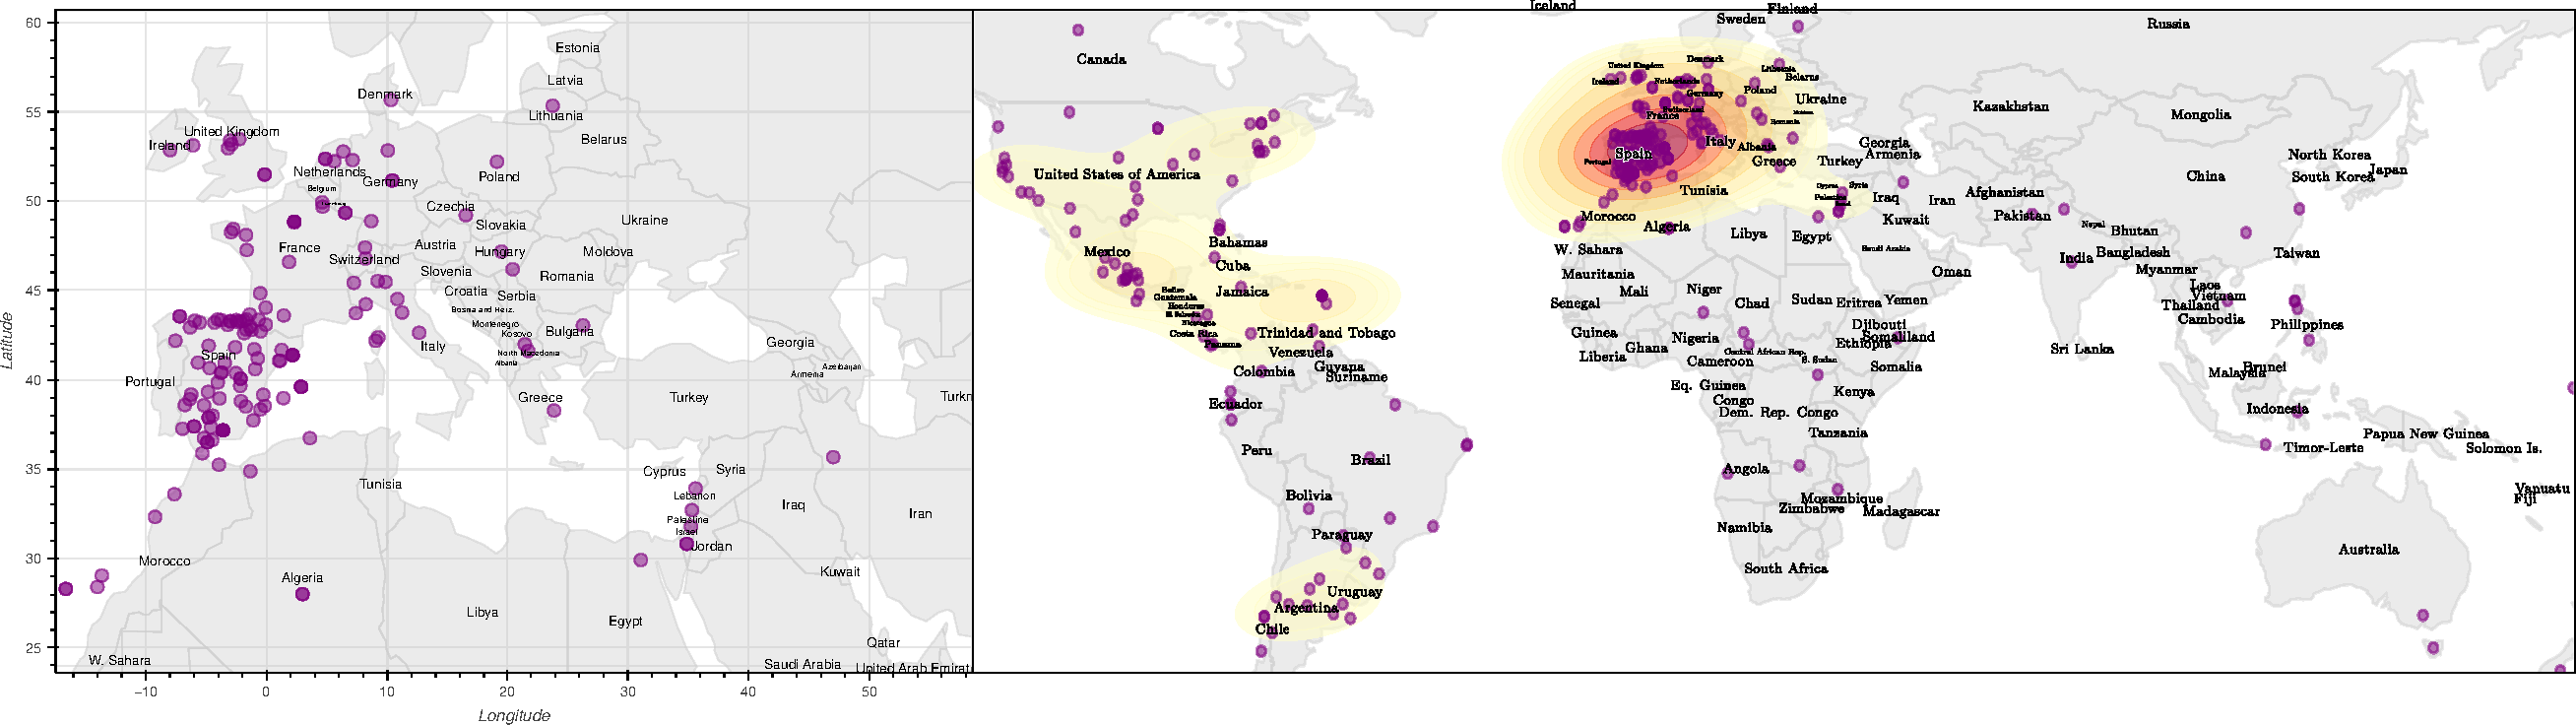
\includegraphics[scale=0.38]{figs/why_passwords/map3.pdf}
    \caption{Map showing passwords that were tagged as location in the labelled \hmail dataset. Location names were extracted from passwords, geolocated and plotted. Southern Europe, especially Spain, is more dense than other regions. This evidence and the prominent language in the \hmail dataset indicates that the passwords came from Spanish speaking regions.\\\srcOwnFig}
    \label{fig:map}
    \vspace{-1em}
\end{figure*}
\newpage
\textbf{\textsc{Location.}}\: We also embed our knowledge of geography and our surroundings into our passwords. We find that the extracted locations are correlated with the language of the users. This indicates that users are more likely to use locations that they are familiar with or are close to. Figure \ref{fig:map} shows the extracted locations on a map. Such a location-based analysis can be beneficial for post-mortem investigations in a data breach and leak. It can help identify the threat vector and the intent of the attacker.

\textbf{\textsc{Age.}}\: The age of the \hmail dataset, 2009, raises the question whether it is still relevant. One can assume that password policies and other unknown factors would have changed our behaviour and therefore the lessons-learnt from the \hmail dataset would not be significant. The machine-labelled \lizardsquad as shown in Table \ref{table:ls-structures} indicates that age of the dataset is less of a factor as we still notice similar patterns in password structures. Password composition policies however do change this pattern but not the underlying human behaviour of embedding information about ourselves and surrounding into these secrets. Moreover, we can still learn from older datasets and one can compare them to a newer labelled datasets in future studies.

 % Studies the characteristics of the labelled data
\ifthenelse{\boolean{pcppapermadweb}}{
    \pagestyle{plain}
\title{Five Word Password Composition Policy}

\author{\IEEEauthorblockN{Sirvan Almasi}
	\IEEEauthorblockA{Imperial College London\\
		sirvan.almasi17@imperial.ac.uk},
	\and
	\IEEEauthorblockN{William J.\,Knottenbelt}
	\IEEEauthorblockA{Imperial College London\\
        w.knottenbelt@imperial.ac.uk}
}


\IEEEoverridecommandlockouts
\makeatletter\def\@IEEEpubidpullup{6.5\baselineskip}\makeatother
\IEEEpubid{\parbox{\columnwidth}{
    {\fontsize{7.5}{7.5}\selectfont Workshop on Measurements, Attacks, and Defenses for the Web (MADWeb) 2025\\
    28 February 2025, San Diego, CA, USA\\
    ISBN 979-8-9894372-9-0\\
    https://dx.doi.org/10.14722/madweb.2025.23020\\
    www.ndss-symposium.org}
}
\hspace{\columnsep}\makebox[\columnwidth]{}}


\maketitle

\begin{abstract}
Password composition policies (PCPs) are critical security rules that govern how users create passwords for online authentication. Despite passwords remaining the primary authentication method online, there is significant disagreement among experts, regulatory bodies, and researchers about what constitutes effective password policies. This lack of consensus has led to high variance in PCP implementations across websites, leaving both developers and users uncertain. Current approaches lack a theoretical foundation for evaluating and comparing different password composition policies. We show that a structure-based policy, such as the three-random words recommended by UK's National Cyber Security Centre (NCSC), can improve password security. We demonstrate this using an empirical evaluation of labelled password datasets and a new theoretical framework. Using these methods we demonstrate the feasibility and security of multi-word password policy and extend the NCSC's recommendation to five words to account for non-uniform word selection. These findings provide an evidence-based framework for password policy development and suggest that current web authentication systems should adjust their minimum word requirements upward while maintaining usability.
\end{abstract}

\section{Introduction}

The lack of consensus on password composition policy (PCP) and the lack of adoption of best practices on the web~\cite{alroomi_measuring_2023, lomchan_comparison_2023, lim_evaluating_2023, maoneke_password_2019, furnell_assessing_2011, woo_survey_2018, lee_password_2022, gerlitz_please_2021} suggests that our knowledge on password security is not yet complete. Although passwords remain the main method of authentication, experts and regulatory bodies disagree fundamentally about what makes a good password policy. State agencies recommend one set of rules, while professional organisations suggest another, and academic researchers advocate for yet different approaches. This lack of consensus reveals a troubling gap in our understanding of password security. What password composition rules should web developers implement to best protect their users?

National organisations such as NIST~(US)~\cite{nist2024} and NCSC~(UK)~\cite{ncsc2024} provide similar guidance on PCP, UK's NCSC additionally recommends minimum of three word password structure. This paper is most interested in structure related policies to enhance user secret security--should a system or web admin recommend such three word password structure policies? In this paper, we develop a model that allows us to reason analytically about PCPs. Using this, we tackle the PCP recommended by the UK's NCSC (minimum of three random words). We present a novel theoretical framework for analysing password composition policies, bridging the gap between security requirements and user behaviour.

The gap between research and practice compounds the inconsistency in the PCP recommendation. Consider Dropbox, which developed \zxcvbn Password Strength Meter (PSM). Despite creating this tool, which has 14.7K Github stars and has been validated by independent research~\cite{wang_no_2023}, Dropbox's own web authentication policy contradicts current best practices. Their website requires passwords with a minimum of eight characters, one letter, one digit, and one symbol. Even more concerning, they do not appear to use their own PSM. \zxcvbn has some weaknesses; it awards its maximum score of 4/4 to \password{girlsruledaworld} and a strong 3/4 to \password{asdf1fdsa1}---passwords that we would consider vulnerable as they are common phrases or sequences.

\textbf{\textsc{Threat Scenario.}} We assume that some users will choose memorable passwords, eschewing password managers or WebAuthn alternatives. Although password managers offer stronger security, our model addresses the reality that many users, from a broad population, will rely on human-generated passwords. Passwords are also useful in offline and air-gapped systems too where out-of-band systems are limited. Therefore, system and web admins have to consider such scenarios. We therefore analyse password security against the most challenging threat model: an offline attack where adversaries can make unlimited guessing attempts without rate limiting.
\vspace*{0.25cm}

\textbf{\textsc{Our Contributions are as Follows:}}
\begin{itemize}
    \item Empirical validation of a structure-based password policy in addition to existing policies. This provides quantitative support for existing password composition recommendations, particularly the NCSC's three-word policy
    \item A formal mathematical model describing the recommended number of words to mitigate user behaviours such as choosing words from a non-uniform distribution.
\end{itemize}

\vspace*{0.25cm}

This work addresses core areas of web security, and our results provide actionable insights for improving password policies across web platforms while maintaining usability. Our findings and insights provide immediate applications for system and web admins. Our work also provides a theoretical and reasoning basis for future password composition policy development and research.

\newpage
\section{Background}
\label{sec::chp4::background}

\textbf{\textsc{Password\;Strength.}}\;This metric measures the difficulty of guessing or cracking a password. However, there is no consensus on how to quantify such difficulty. Some experts use dictionary-based methods, while others rely on probabilistic deep-learning based approaches. Nonetheless, certain lower-bound measures are widely accepted, such as the minimum number of characters required to prevent brute-force attacks.

Shannon's entropy (Eq. \ref{eq:entropy}) quantifies the uncertainty or information content associated with a random variable. \begin{equation}\label{eq:entropy}
H(X) = -\sum_{x\in\mathcal{X}}^{} p(x) \log p(x)
\end{equation} In the context of password strength, it measures how unpredictable or "random" a password is. The higher the entropy, the more difficult the password is to guess, making it stronger. This metric estimates the minimum number of bits required to encode the password. However, the entropy measure for passwords is often given in the form of $\log_2(R^L)$, where $R$ represents the total number of characters in the character sets used in the password, and $L$ is the length of the password.

The limitation of $\log_2(R^L)$ is that it assumes all $R$ characters are equally likely, disregarding the dependency between characters in human-chosen passwords. This approach oversimplifies, as passwords like \password{8zm!U6gNL\%} and \password{p4\$sW0rd1!} are calculated to have the same entropy. However, such an assumption is unrealistic, as the latter password is essentially the word \textit{password} with predictable transformations.

\textbf{\textsc{Password Composition Policies (PCP).}}\: PCP is set of rules, often in natural language, that only allows the user to sample from a password space that is assumed to be resistant to guessing attacks. The \textit{National Cyber Security Centre (NCSC)}~\cite{ncsc2024} in the UK and the \textit{National Institute of Standards and Technology (NIST)}~\cite{nist2024} in the USA are leading authorities in cyber-security. Their recommendations, particularly on password policies, should serve as standards or benchmarks in the field. Specifically, the NCSC advocates for the use of three random words~\cite{McCormackthreerandom} and advises against mandatory password complexity requirements~\cite{password_policy_ncsc}. This approach, detailed in~\cite{Kate_2021}, is based on the principle that a sequence of three random words is both easier for users to remember and sufficiently complex to deter unauthorised access, striking a balance between security and user convenience. This three word and structure-based PCP is conditioned on the following:

\begin{itemize}[itemsep=0pt, parsep=0pt, leftmargin=11pt]
    \item \textsc{\textbf{Length}}. To satisfy the minimum length requirements.
    \item \textsc{\textbf{Impact}}. Easy to adopt and understand.
    \item \textsc{\textbf{Novelty}}. Unlikely to find it in a breached database.
    \item \textsc{\textbf{Usability}}. More likely to be remembered.
\end{itemize}
\label{jmp::chp4::ncsc-pcp}

NIST's \cite{Grassi_Garcia_Fenton_2020} PCP is as follows. Passwords should have a minimum length of 8 characters, but systems should support more than 64 characters. It is advised to compare the selected password against prior breach data, dictionary entries, and repetitive patterns. Context-specific terms should also be considered. Additionally, users should be aided with strength meters to gauge password robustness. While rate limiting should be enforced during authentication attempts, use of specific composition rules is discouraged.
OWASP \cite{owasp_owasp_2024} follows the recommendations set by NIST.

\textbf{\textsc{passwordNinja Dataset \cite{almasi2024passwordninja}}} is a human and machine labelled datasets that has decomposed password strings into its finer constituents. For example, the password \password{0rwell1984} would be structured as follows.
\[
\begin{aligned}
& \underbrace{\text{\password{0rwell}}}_{\text{word }(w)} \underbrace{\text{\password{1984}}}_{\text{date}} \\[10pt]
\end{aligned}
\vspace*{-0.3cm}
\]
The \fun{passwordNinja}~\cite{almasi2024passwordninja} dataset is composed of a complete \hmail and \lizardsquad breached passwords from 2009 and 2015 respectively. The \hmail dataset, which leaked in 2009~\cite{johnson_hotmail_2009}, comprises \num{8929} records of passwords. Public sources indicate that these passwords were procured through phishing. Abundant evidence within the dataset supports this claim. For instance, we observe numerous passwords with inverted capitalisation and similar passwords that contain typos, suggesting that users might have unintentionally activated \texttt{CAPS\;LOCK}. The \lizardsquadnocite dataset contains \num{11808} records.
}{}
\vspace*{-0.7cm}
\section{Password\;Composition\;Policy}
\vspace*{-0.4cm}
\label{sec::chp4::pcp}
\begin{figure*}[ht]
    \centering
    \begin{subfigure}[b]{0.45\linewidth}
        \centering
        \scalebox{1}{\input{figs/why_passwords/word_freq_loglog}}
        \caption{Unique Words}
        \label{fig:word_freq_loglog}
    \end{subfigure}
    \hspace{0.5cm} % Space between the two figures
    \begin{subfigure}[b]{0.45\linewidth}
        \centering
        \scalebox{1}{\input{figs/why_passwords/structure_loglog}}
        \caption{Structures}
        \label{fig:structure_loglog}
    \end{subfigure}
    \caption{Charts showing the log-log plot of word and structure against their respective rank for the \hmail dataset. Words are from extracted unique passwords. The distribution of both words and structure exhibit a power law similar to Zipf's law.}
    \label{fig:log-log-charts}
    %\vspace{-1.5em} % Adjust the negative value to reduce the gap
\end{figure*}

\begin{table*}[h]
    \centering
    %\footnotesize
    \scriptsize
    
    \caption{The table presents the top 25 labelled password structures from the passwordNinja \cite{almasi2024passwordninja} dataset, accounting for 5\,032 (69.5\%) of the labelled dataset. Hashcat \cite{steube_hashcat_2023} benchmarks indicate the performance of consumer hardware in a hybrid attack. The dictionary size for $\bm{w}$ (words) and $\bm{n}$ (numbers) is set at $5\times 10^5$. \zxcvbn serves as a password strength meter, with scores ranging from 0 to 4, and guess estimates are log based.}
    \label{table:structures}
    \setlength\tabcolsep{1pt} % default value: 6pt
    {\renewcommand{\arraystretch}{0.3}% for the vertical padding
    \begin{tabular}{rllc|cccc|cc}
    % \toprule
     & & \multicolumn{2}{c}{Frequency}  & \multicolumn{4}{c}{Hashcat using Nvidia RTX 4090} & \multicolumn{2} {c}{\zxcvbnnocite Mean} \\\cmidrule{3-4} \cmidrule{5-10}
    \textbf{Structure} & \textbf{$log$ perm'} & \textbf{Count} & \textbf{\%} & \textbf{MD5} & \textbf{PBKDF2-sha256} & \textbf{scrypt} & \textbf{bcrypt-sha512} & \textbf{Score} & \textbf{Guesses} \\
    \midrule
w & \DrawLengthBarThick{4.7} & \DrawLengthBarThick{15.2} 1520 & 21.0 & $\sim0$ & 0.1 s & 1 min & 4 min & 1.3 & 5.36 \\
n & \DrawLengthBarThick{4.7} & \DrawLengthBarThick{8.11} 811 & 11.2 & $\sim0$ & 0.1 s & 1 min & 4 min & 1.0 & 4.72 \\
nd & \DrawLengthBarThick{5.6} & \DrawLengthBarThick{0.58} 58 & 0.8 & $\sim0$ & 0.6 s & 12 min & 42 min & 1.4 & 5.68 \\
wd & \DrawLengthBarThick{5.6} & \DrawLengthBarThick{0.91} 91 & 1.3 & $\sim0$ & 0.6 s & 12 min & 42 min & 1.5 & 5.97 \\
nl & \DrawLengthBarThick{5.9} & \DrawLengthBarThick{0.33} 33 & 0.5 & $\sim0$ & 1.5 s & 30 min & 2 h & 1.2 & 5.09 \\
wdd & \DrawLengthBarThick{6.4} & \DrawLengthBarThick{2.94} 294 & 4.1 & $\sim0$ & 5.6 s & 2 h & 7 h & 1.8 & 6.69 \\
ndd & \DrawLengthBarThick{6.4} & \DrawLengthBarThick{2.21} 221 & 3.1 & $\sim0$ & 5.6 s & 2 h & 7 h & 1.6 & 6.33 \\
nddd & \DrawLengthBarThick{7.2} & \DrawLengthBarThick{0.71} 71 & 1.0 & $\sim0$ & 56.4 s & 19 h & 3 day & 1.7 & 6.37 \\
wddd & \DrawLengthBarThick{7.2} & \DrawLengthBarThick{0.91} 91 & 1.3 & $\sim0$ & 56.4 s & 19 h & 3 day & 1.9 & 6.84 \\
wsdd & \DrawLengthBarThick{7.6} & \DrawLengthBarThick{0.29} 29 & 0.4 & $\sim0$ & 3 min & 3 day & 9 day & 2.0 & 7.28 \\
ddddw & \DrawLengthBarThick{8.1} & \DrawLengthBarThick{0.35} 35 & 0.5 & $\sim0$ & 9 min & 8 day & 29 day & 2.4 & 7.95 \\
wdddd & \DrawLengthBarThick{8.1} & \DrawLengthBarThick{1.74} 174 & 2.4 & $\sim0$ & 9 min & 8 day & 29 day & 2.3 & 7.59 \\
ndddd & \DrawLengthBarThick{8.1} & \DrawLengthBarThick{2.05} 205 & 2.8 & $\sim0$ & 9 min & 8 day & 29 day & 2.0 & 6.90 \\
nn & \DrawLengthBarThick{9.5} & \DrawLengthBarThick{3.76} 376 & 5.2 & 1.5 s & 8 h & 1 yr & 4 yr & 2.0 & 6.91 \\
ww & \DrawLengthBarThick{9.5} & \DrawLengthBarThick{4.57} 457 & 6.3 & 1.5 s & 8 h & 1 yr & 4 yr & 2.0 & 7.04 \\
nw & \DrawLengthBarThick{9.5} & \DrawLengthBarThick{0.3} 30 & 0.4 & 1.5 s & 8 h & 1 yr & 4 yr & 2.2 & 7.51 \\
ndddddd & \DrawLengthBarThick{9.7} & \DrawLengthBarThick{0.51} 51 & 0.7 & 3.0 s & 16 h & 2 yr & 8 yr & 2.5 & 8.05 \\
wdddddd & \DrawLengthBarThick{9.7} & \DrawLengthBarThick{0.33} 33 & 0.5 & 3.0 s & 16 h & 2 yr & 8 yr & 2.8 & 8.84 \\
wwdd & \DrawLengthBarThick{11.1} & \DrawLengthBarThick{0.58} 58 & 0.8 & 3 min & 33 day & 111 yr & 402 yr & 2.9 & 8.97 \\
nndd & \DrawLengthBarThick{11.1} & \DrawLengthBarThick{0.38} 38 & 0.5 & 3 min & 33 day & 111 yr & 402 yr & 3.2 & 9.62 \\
wwdddd & \DrawLengthBarThick{12.8} & \DrawLengthBarThick{0.33} 33 & 0.5 & 4 h & 9 yr & $1.11 \times 10^{4}$ yr & $4.02 \times 10^{4}$ yr & 3.3 & 9.81 \\
nwn & \DrawLengthBarThick{14.2} & \DrawLengthBarThick{0.41} 41 & 0.6 & 9 day & 447 yr & $5.56 \times 10^{5}$ yr & $2.01 \times 10^{6}$ yr & 3.0 & 8.88 \\
www & \DrawLengthBarThick{14.2} & \DrawLengthBarThick{1.65} 165 & 2.3 & 9 day & 447 yr & $5.56 \times 10^{5}$ yr & $2.01 \times 10^{6}$ yr & 3.0 & 9.26 \\
nww & \DrawLengthBarThick{14.2} & \DrawLengthBarThick{0.35} 35 & 0.5 & 9 day & 447 yr & $5.56 \times 10^{5}$ yr & $2.01 \times 10^{6}$ yr & 2.7 & 8.18 \\
nnn & \DrawLengthBarThick{14.2} & \DrawLengthBarThick{0.27} 27 & 0.4 & 9 day & 447 yr & $5.56 \times 10^{5}$ yr & $2.01 \times 10^{6}$ yr & 3.3 & 9.95 \\
wwww & \DrawLengthBarThick{15.3} & \DrawLengthBarThick{0.55} 55 & 0.8 & 171 day & $8.70 \times 10^{3}$ yr & $1.08 \times 10^{7}$ yr & $3.91 \times 10^{7}$ yr & 3.5 & 11.24 \\
\bottomrule
    \end{tabular}
    } %% vertical padding
\end{table*}
\ifthenelse{\boolean{pcppapermadweb}}{}{
\begin{table*}[!ht]
    \centering
    %\footnotesize
    \scriptsize
    \caption{The table presents the top 25 labelled password structures from the Lizard-Squad dataset. Hashcat \cite{steube_hashcat_2023} benchmarks indicate the performance of consumer hardware in a hybrid attack. The dictionary size for $\bm{w}$ (words) and $\bm{n}$ (numbers) is set at $5\times 10^5$. \zxcvbn serves as a password strength meter, with scores ranging from 0 to 4, and guess estimates are log based.}
    \label{table:ls-structures}
    \setlength\tabcolsep{1pt} % default value: 6pt
    {\renewcommand{\arraystretch}{0.3}% for the vertical padding
    \begin{tabular}{rllc|cccc|cc}
    % \toprule
     & & \multicolumn{2}{c}{Frequency}  & \multicolumn{4}{c}{Hashcat using Nvidia RTX 4090} & \multicolumn{2} {c}{\zxcvbnnocite Mean} \\\cmidrule{3-4} \cmidrule{5-10}
    \textbf{Structure} & \textbf{$log$ perm'} & \textbf{Count} & \textbf{\%} & \textbf{MD5} & \textbf{PBKDF2-sha256} & \textbf{scrypt} & \textbf{bcrypt-sha512} & \textbf{Score} & \textbf{Guesses} \\
    \midrule
w & \DrawLengthBarThick{4.7} & \DrawLengthBarThick{5.94} 594 & 5.5 & $\sim0$ & 0.1 s & 1 min & 4 min & 0.9 & 4.24 \\
n & \DrawLengthBarThick{4.7} & \DrawLengthBarThick{1.89} 189 & 1.7 & $\sim0$ & 0.1 s & 1 min & 4 min & 0.8 & 4.13 \\
wd & \DrawLengthBarThick{5.6} & \DrawLengthBarThick{2.54} 254 & 2.3 & $\sim0$ & 0.6 s & 12 min & 42 min & 1.2 & 5.06 \\
nd & \DrawLengthBarThick{5.6} & \DrawLengthBarThick{1.35} 135 & 1.2 & $\sim0$ & 0.6 s & 12 min & 42 min & 1.5 & 5.71 \\
wdd & \DrawLengthBarThick{6.4} & \DrawLengthBarThick{6.67} 667 & 6.1 & $\sim0$ & 5.6 s & 2 h & 7 h & 1.4 & 5.64 \\
ndd & \DrawLengthBarThick{6.4} & \DrawLengthBarThick{4.57} 457 & 4.2 & $\sim0$ & 5.6 s & 2 h & 7 h & 1.4 & 5.85 \\
wddd & \DrawLengthBarThick{7.2} & \DrawLengthBarThick{7.36} 736 & 6.8 & $\sim0$ & 56.4 s & 19 h & 3 day & 1.6 & 6.10 \\
nddd & \DrawLengthBarThick{7.2} & \DrawLengthBarThick{4.09} 409 & 3.8 & $\sim0$ & 56.4 s & 19 h & 3 day & 1.6 & 6.04 \\
wdddd & \DrawLengthBarThick{8.1} & \DrawLengthBarThick{4.65} 465 & 4.3 & $\sim0$ & 9 min & 8 day & 29 day & 1.7 & 6.41 \\
ndddd & \DrawLengthBarThick{8.1} & \DrawLengthBarThick{3.59} 359 & 3.3 & $\sim0$ & 9 min & 8 day & 29 day & 1.7 & 6.18 \\
nddddd & \DrawLengthBarThick{8.9} & \DrawLengthBarThick{0.58} 58 & 0.5 & 0.3 s & 2 h & 81 day & 293 day & 1.8 & 6.51 \\
wddddd & \DrawLengthBarThick{8.9} & \DrawLengthBarThick{0.84} 84 & 0.8 & 0.3 s & 2 h & 81 day & 293 day & 2.0 & 6.89 \\
nn & \DrawLengthBarThick{9.5} & \DrawLengthBarThick{1.39} 139 & 1.3 & 1.5 s & 8 h & 1 yr & 4 yr & 1.6 & 6.03 \\
nw & \DrawLengthBarThick{9.5} & \DrawLengthBarThick{0.26} 26 & 0.2 & 1.5 s & 8 h & 1 yr & 4 yr & 1.8 & 6.42 \\
ww & \DrawLengthBarThick{9.5} & \DrawLengthBarThick{6.66} 666 & 6.1 & 1.5 s & 8 h & 1 yr & 4 yr & 1.5 & 5.84 \\
ndddddd & \DrawLengthBarThick{9.7} & \DrawLengthBarThick{0.51} 51 & 0.5 & 3.0 s & 16 h & 2 yr & 8 yr & 2.3 & 7.24 \\
wdddddd & \DrawLengthBarThick{9.7} & \DrawLengthBarThick{0.52} 52 & 0.5 & 3.0 s & 16 h & 2 yr & 8 yr & 1.9 & 6.92 \\
nnd & \DrawLengthBarThick{10.3} & \DrawLengthBarThick{0.73} 73 & 0.7 & 15.2 s & 3 day & 11 yr & 40 yr & 2.4 & 7.82 \\
wwd & \DrawLengthBarThick{10.3} & \DrawLengthBarThick{2.31} 231 & 2.1 & 15.2 s & 3 day & 11 yr & 40 yr & 2.1 & 7.18 \\
wwdd & \DrawLengthBarThick{11.1} & \DrawLengthBarThick{3.07} 307 & 2.8 & 3 min & 33 day & 111 yr & 402 yr & 2.4 & 7.61 \\
nndd & \DrawLengthBarThick{11.1} & \DrawLengthBarThick{0.86} 86 & 0.8 & 3 min & 33 day & 111 yr & 402 yr & 2.8 & 8.64 \\
wwddd & \DrawLengthBarThick{12.0} & \DrawLengthBarThick{2.33} 233 & 2.1 & 25 min & 326 day & $1.11 \times 10^{3}$ yr & $4.02 \times 10^{3}$ yr & 2.5 & 7.93 \\
nnddd & \DrawLengthBarThick{12.0} & \DrawLengthBarThick{0.48} 48 & 0.4 & 25 min & 326 day & $1.11 \times 10^{3}$ yr & $4.02 \times 10^{3}$ yr & 2.9 & 8.96 \\
nndddd & \DrawLengthBarThick{12.8} & \DrawLengthBarThick{0.28} 28 & 0.3 & 4 h & 9 yr & $1.11 \times 10^{4}$ yr & $4.02 \times 10^{4}$ yr & 3.1 & 9.54 \\
wwdddd & \DrawLengthBarThick{12.8} & \DrawLengthBarThick{0.76} 76 & 0.7 & 4 h & 9 yr & $1.11 \times 10^{4}$ yr & $4.02 \times 10^{4}$ yr & 2.8 & 8.39 \\
www & \DrawLengthBarThick{14.2} & \DrawLengthBarThick{2.1} 210 & 1.9 & 9 day & 447 yr & $5.56 \times 10^{5}$ yr & $2.01 \times 10^{6}$ yr & 2.3 & 7.33 \\
wwwd & \DrawLengthBarThick{15.0} & \DrawLengthBarThick{0.42} 42 & 0.4 & 88 day & $4.47 \times 10^{3}$ yr & $5.56 \times 10^{6}$ yr & $2.01 \times 10^{7}$ yr & 2.3 & 7.45 \\
wwwdd & \DrawLengthBarThick{15.9} & \DrawLengthBarThick{0.42} 42 & 0.4 & 2 yr & $4.47 \times 10^{4}$ yr & $5.56 \times 10^{7}$ yr & $2.01 \times 10^{8}$ yr & 3.1 & 9.43 \\
wwwddd & \DrawLengthBarThick{16.7} & \DrawLengthBarThick{0.39} 39 & 0.4 & 24 yr & $4.47 \times 10^{5}$ yr & $5.56 \times 10^{8}$ yr & $2.01 \times 10^{9}$ yr & 2.9 & 9.02 \\
wwww & \DrawLengthBarThick{18.9} & \DrawLengthBarThick{0.54} 54 & 0.5 & $1.21 \times 10^{4}$ yr & $2.24 \times 10^{8}$ yr & $2.78 \times 10^{11}$ yr & $1.00 \times 10^{12}$ yr & 3.1 & 9.77 \\
\bottomrule
    \end{tabular}
    } %% vertical padding
\end{table*}
}

%To demonstrate the utility of the labelled dataset and its impact we will test how well it can help us create usable and effective Password Composition Policies (PCP).

There is a lack of consensus on password composition policy amongst industry experts, academics and government agencies. This has created some confusion which is evident by the fact that most web applications do not follow any best practices~\cite{alroomi_measuring_2023, lomchan_comparison_2023, lim_evaluating_2023, maoneke_password_2019, furnell_assessing_2011, woo_survey_2018, lee_password_2022, gerlitz_please_2021}. This raises the question which PCP is the \textit{right} one? Specifically, should we have a structure-based policy as recommended by UK's NCSC?

To answer this question we pay particular attention to the  \hyperref[jmp::chp4::ncsc-pcp]{NCSC's PCP} of three random words. We first develop a mathematical model that incorporates password structures, this is novel and enabled by the \pwdninja dataset.

\subsection{Empirical Evaluation}
To analyse how the password structure affects security, we draw on the data set \pwdninja as described in the previous section. This dataset provides something previously unavailable to researchers: individually labelled passwords that reveal their structural composition. This labelling is essential for our analysis, as it allows us to systematically evaluate how different password structures influence the security strength.

Our analysis of password datasets reveals several key vulnerabilities in how users choose passwords. First, users select words from a highly biased distribution, making passwords more predictable (Figure~\ref{fig:word_freq_loglog}). Second, commonly used password structures contain patterns that attackers can exploit using techniques such as Probabilistic Context-free Grammar (\pcfg) or mask attack mode in \hashcat.

As shown in Table\;\ref{table:structures}, single words ($w$) and names ($n$) dominate password structures, making them vulnerable to dictionary attacks. The effectiveness of these attacks varies by hash function; our tests using consumer hardware demonstrate significantly different cracking times across hash functions. A newer dataset (\lizardsquad 2015) shows similar structural patterns (More detail in Table~\ref{table:ls-structures}.)

However, passwords containing multiple words (such as $w^4$ structures) demonstrate much stronger security, resisting hybrid attacks even when hashed with MD5. Yet this strength depends critically on word choice. When users select related words or popular phrases (such as song lyrics), passwords become more predictable. For example, the phrase \texttt{"mira que eres canalla"} is vulnerable, even though it is made up of four words. This is because it originates from Mexican folk music.

To maximise security, users should select words with minimal semantic or probabilistic relationships in their sequence. This prevents attackers from using language models to predict subsequent words in multi-word passwords or passphrases.

Our analysis of the \pwdninja datasets supports the NCSC guidelines. Testing with \zxcvbn (Figure~\ref{fig:heatmap_structure} and Table~\ref{table:bin4}) confirms that multi-word passwords improve the security of human-chosen and memorable passwords.

\begin{table}
    \centering
    \caption{Top 10 password structures for each \zxcvbn score of 3 an 4. These are the password structures that are categorised in the most secure bin (4) by the \zxcvbnnocite algorithm; Avg Guesses is the \zxcvbnnocite \texttt{guesses\_log10}.}
    \label{table:bin4}
    \setlength\tabcolsep{1pt} % default value: 6pt
    {\renewcommand{\arraystretch}{0.5}% for the vertical padding
    \begin{tabular}{ccc|c|c}
    \toprule
    \textbf{Structure} & & \textbf{Count} & \textbf{Avg Guesses} & \textbf{Avg Length} \\
    \midrule
        \multicolumn{2}{c}{\textbf{zxcvbn score = 4}}  & & & \\
        r2 & $r2$ 	 & 160 & 12.6 & 14 \\
        www & $w^3$ 	 & 57 & 12.1 & 14 \\
        ww & $w^2$ 	 & 48 & 12.0 & 14 \\
        wwww & $w^4$ 	 & 34 & 13.1 & 15 \\
        w & $w$ 	 & 25 & 11.3 & 12 \\
        nn & $n^2$ 	 & 24 & 11.2 & 13 \\
        wdddd & $wd^4$ 	 & 19 & 11.6 & 12 \\
        wwdddd & $w^2d^4$ 	 & 16 & 11.3 & 14 \\
        nndd & $n^2d^2$ 	 & 15 & 11.5 & 13 \\
        ndddd & $nd^4$ 	 & 14 & 10.8 & 12 \\
        \midrule
        \multicolumn{2}{c}{\textbf{zxcvbn score = 3}}  & & & \\
        r2 & $r2$ 	 & 185 & 8.9 & 10 \\
        w & $w$ 	 & 100 & 8.8 & 10 \\
        ww & $w^2$ 	 & 86 & 8.8 & 11 \\
        nn & $n^2$ 	 & 77 & 8.8 & 11 \\
        www & $w^3$ 	 & 62 & 9.1 & 11 \\
        wdddd & $wd^4$ 	 & 44 & 8.8 & 11 \\
        ndddd & $nd^4$ 	 & 43 & 8.7 & 10 \\
        wdd & $wd^2$ 	 & 38 & 9.0 & 10 \\
        wwdd & $w^2d^2$ 	 & 31 & 9.1 & 11 \\
        n & $n$ 	 & 26 & 8.9 & 10 \\
    \bottomrule
    \end{tabular}
    } %% vertical padding 
    \vspace{-1em}
\end{table}
\vspace*{-0.2cm}
\subsection{Theoretical Evaluation}
\vspace*{-0.1cm}
\subsubsection{Password Structure Probability}
   
   Let \( S \) denote the structure of a password, where \( S(p) = (e_1, e_2, \dots, e_n) \) and each \( e_i \in \Sigma \) (e.g., \( \Sigma = \{w, n, d, s, \dots\} \)). The probability of a structure \( S \) is given by $P(S) = P(e_1, e_2, \dots, e_n)$. Assuming dependence between the elements in the structure, this can be expressed as:
   \begin{equation}
   P(S) = P(e_1) \prod_{i=2}^{n} P(e_i \mid e_{i-1})
   \end{equation}

\subsubsection{Combined Relationship Probability}

If $e_i$ represents the type of the element, then let $\hat{e_i}$ represent the instance of the element, e.g. $\hat{e} \rightarrow$ \textit{password} if $e=w$ (i.e. a word). We can represent both structure and instance relationships using a joint distribution. For a password $p$ with elements $(e_1, ..., e_n)$, we can define:
\begin{align}
 P(p) &=P(S(p),\,E(p)) \\
      &= P(S(p)) \, P(E(p) \mid S(p))
 \label{eq::chp4::p(p)}
\end{align}
Where $E(p)$ represents the specific element instances.
\begin{equation}
P(E(p) \mid S(p)) = P(\hat{e}_1) \, \prod_{i=2}^n P(\hat{e}_i \mid \hat{e}_{i-1},S(p))
\end{equation}
The final equation simplified is:
   \begin{equation}
    P(p) = P(e_1) P(\hat{e}_1) \prod_{i=2}^{n} [P(e_i \mid e_{i-1}) P(\hat{e}_i \mid \hat{e}_{i-1},S(p))]
   \end{equation}

% Calculate the $H(S)$ for \hmail dataset.
% TODO: Information theory based password probability 
%\subsubsection{Information Theoretic}
%
%\begin{multline}
%P(p) = P(S(p)) \cdot \psi(E(p)) \\
%\psi(E(p)) = \exp \left(\sum_{i=1}^{n-1} I(e_i; e_{i+1})\right) \\
%I(e_i; e_{i-1}) = \log \frac{P(e_i, e_{i-1})}{P(e_i)P(e_{i+1})} \\
%\end{multline}

   % Let \( R(e_i, e_j) \) represent the semantic relationship between elements \( e_i \) and \( e_j \). The probability that a pair of elements \( (e_i, e_j) \) holds a specific semantic relationship can be modelled as $P(R(e_i, e_j) \mid e_i, e_j)$. For a sequence of elements, the joint probability of all semantic relationships can be represented as:
   % \begin{equation}
   % P(R \mid S) = \prod_{1 \leq i < j \leq n} P(R(e_i, e_j) \mid e_i, e_j)
   % \end{equation}

% \subsubsection{Combined Password Probability}
%    
%    The overall probability of a password \( p \) with structure \( S(p) \) and semantic relationships \( R \) is the product of the structure probability and the semantic relationship probability:
%    \begin{equation}
%    P(p) = P(S(p)) \cdot P(R \mid S(p))
%    \end{equation}
%    
%    Expanding this, we have:
%    \begin{equation}
%    P(p) = \prod_{i=1}^{n} P(e_i) \, \prod_{1 \leq i < j \leq n} P(R(e_i, e_j) \mid e_i, e_j)
%    \end{equation}

%\subsubsection{Optimization Objective for Password Policy}
%   
%   To determine the ideal password composition policy, we aim to maximize the entropy of the password distribution, thereby ensuring maximum unpredictability. The entropy \( H \) of the password distribution is given by:
%   \begin{equation}
%       H(P) = - \sum_{p \in \mathcal{P}} P(p) \log P(p)
%    \label{eq::chp4::hp}
%   \end{equation}
%   %Substituting the expression for \( P(p) \):
%   %\begin{multline}
%   % H(P) = - \sum_{p \in \mathcal{P}}  P(e_1) \prod_{i=2}^{n} P(e_i \mid e_{i-1}) P(\hat{e}_1) \, \prod_{i=2}^n P(\hat{e}_i \mid \hat{e}_{i-1},S(p))
%   %\end{multline}
%   % \begin{multline}
%   % H(P) = - \sum_{p \in \mathcal{P}} \left( \prod_{i=1}^{n} P(e_i) \right) \left( \prod_{1 \leq i < j \leq n} P(R(e_i, e_j) \mid e_i, e_j) \right) \\ \log \left[  \prod_{i=1}^{n} P(e_i) \cdot  \prod_{1 \leq i < j \leq n} P(R(e_i, e_j) \mid e_i, e_j)  \right]
%   % \end{multline}
%   
%   The optimization problem can then be formulated as:
%   \begin{equation}
%   \max_{P(S), P(E \mid S)} H(P)
%   \end{equation}
%   
%   Subject to any necessary constraints, such as minimum structure complexity or specific semantic relationships to be avoided.

%\subsubsection{Entropy}
%\begin{multline}
%H(p) = -\sum_p P(p)\log_2\left(P(e_1)P(\bar{e}_1)\prod_{i=2}^n [P(e_i|e_{i-1})P(\bar{e}_i|\bar{e}_{i-1}, S(p))]\right) \\
%= -\sum_p P(p)\left[\log_2 P(e_1) + \log_2 P(\bar{e}_1) + \sum_{i=2}^n \log_2 P(e_i|e_{i-1}) + \sum_{i=2}^n \log_2 P(\bar{e}_i|\bar{e}_{i-1}, S(p))\right]
%\end{multline}

\subsubsection{Incorporating NCSC's Recommendation}
Aligning with the NCSC's recommendation of using at least three random words, we define a specific structure $S^*$ where $S^*~=~(w,~w,~w)$. We assume a fixed structure of just three words, thus $P(S^*) = 1$. Using Eq.~\ref{eq::chp4::p(p)}, we are left with $P(p~\mid~S^*)~=~P(E(p)~\mid~S(p))$. We also assume that the words are chosen independently. Thus, we have:
\begin{equation}
P(p \mid S^*) = \prod_{i=1}^{3} P(w_i)
\end{equation}
   %  Let \( w \) denote a word from the vocabulary \( \mathcal{W} \), assume that words are chosen 
   %  \( P(w) = \frac{1}{|\mathcal{W}|} \)
   
   
   %The probability of this structure is $P(S^*) = \prod_{i=1}^{3} P(w)$. And the combined probability for passwords following this structure with no semantic relationships (i.e., words are chosen independently) is:
   %\begin{equation}
   %P(p \mid S^*) = \prod_{i=1}^{3} P(w_i)
   %\end{equation}

\subsection{Non-uniform NCSC PCP}
\vspace*{-0.1cm}
In practice humans do not select words at random and the \pwdninja~\cite{almasi2024passwordninja} dataset shows that the selection of words follows a power-law like distribution. This has significant implications for the NCSC's recommendation of using at least three random words for password composition. Below is a mathematical framework to model this scenario and assess the impact on the password composition policy.

\vspace*{-0.5cm}
\subsubsection{Word Frequency Distribution}
\vspace*{-0.25cm}
   Let \( w \) denote a word from the vocabulary \( \mathcal{W} \). Under Zipf's law, the probability \( P(w) \) of selecting the \( r \)-th most frequent word is given by:
   \begin{equation}
   P(w_r) = \frac{1 / r^s}{\sum_{k=1}^{|\mathcal{W}|} 1 / k^s}
   \end{equation}
   where \( s \) is the exponent characterizing the distribution (typically \( s \approx 1 \) for natural languages).

   % Alternatively, under a Pareto distribution, the probability density function (for continuous variables) is:
   % \[
   % f(w) = \frac{\alpha k^\alpha}{w^{\alpha + 1}} \quad \text{for } w \geq k
   % \]
   % where \( \alpha > 0 \) is the shape parameter and \( k \) is the scale parameter.

% \subsubsection{Password Structure Probability with Zipf's Law}
   For a password \( p \) consisting of \( n \) words \( (w_1, w_2, \dots, w_n) \) selected independently according to Zipf's law, the structure probability \( P(S) \) where \( S = (w, w, \dots, w) \) is:
   \begin{equation}
   P(S) = \prod_{i=1}^{n} P(w_i) = \prod_{i=1}^{n} \frac{1 / r_i^s}{\sum_{k=1}^{|\mathcal{W}|} 1 / k^s}
   \end{equation}
   where \( r_i \) is the rank of the \( i \)-th word.

\subsubsection{Entropy of the Password Distribution under Zipf's Law}

   The entropy \( H \) of the password distribution. Substituting \( P(p) \) with the structure probability:
   \begin{equation}
   H = - \sum_{w_i \in \mathcal{W}}^n \left( \prod_{i=1}^{n} \frac{1 / r_i^s}{\sum_{k=1}^{|\mathcal{W}|} 1 / k^s} \right) \log \left( \prod_{i=1}^{n} \frac{1 / r_i^s}{\sum_{k=1}^{|\mathcal{W}|} 1 / k^s} \right)
   \end{equation}
   
   Simplifying the logarithm:
   %\[
   %H = - \sum_{w_1, w_2, \dots, w_n \in \mathcal{W}} \left( \prod_{i=1}^{n} P(w_i) \right) \left( \sum_{i=1}^{n} \log P(w_i) \right)
   %\]
   \begin{equation}
   H = - \sum_{i=1}^{n} \sum_{w_i \in \mathcal{W}} P(w_i) \log P(w_i) = n \cdot H_{\text{word}}
   \end{equation}
   where \( H_{\text{word}} \) is the entropy per word. We will now use this to draw a comparison with the uniform distribution, which we take to be the theoretical version of the NCSC's PCP.
   %\[
   %H_{\text{word}} = - \sum_{w \in \mathcal{W}} P(w) \log P(w)
   %\]

\subsubsection{Impact on NCSC's Recommendation}
    \begin{figure}
        \centering
        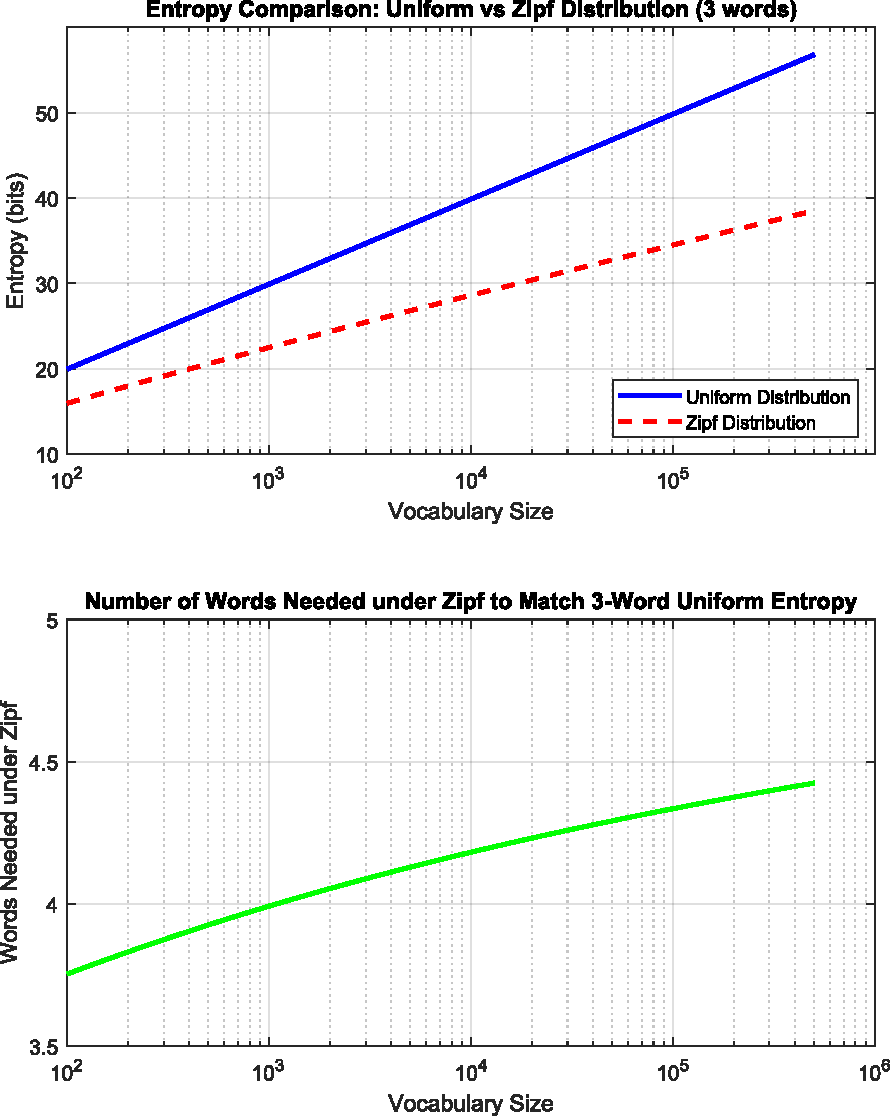
\includegraphics[scale=0.8]{figs/why_passwords/ncsc_threewords_diff.pdf}
        \caption{Chart showing the equivalent number of words required in practice to match the theoretical complexity of the National Cyber Security Centre's (NCSC) password composition policy. The NCSC recommends at least three random words, using our model we show that in practice a minium of 4 words is more secure. \srcOwnFig}
        \label{fig::chp4::zipfslaw-ncsc}
        \vspace*{-0.5cm}
    \end{figure}
   To align the password policy with enhanced entropy under Zipf's law, we need to determine the minimum number of words \( n \) required to achieve a desired entropy \( H_{\text{desired}} \). This can be formulated as:
   \[
n \geq \frac{H_{\text{desired}}}{H_{\text{word}}}
   \]
   Given that \( H_{\text{word}} \) is lower under Zipf's law compared to a uniform distribution (due to the presence of highly probable words), a larger \( n \) may be required to achieve the same entropy.
   
   Under a uniform distribution where each word has \( P(w) = \frac{1}{|\mathcal{W}|} \), the entropy per word is:
   $$H_{\text{word}}^{\text{uniform}} = \log |\mathcal{W}|$$
   Comparing with Zipf's law:
   \[
H_{\text{word}}^{\text{Zipf}} < H_{\text{word}}^{\text{uniform}}
   \]
   
   Zipf's law requires more words than a uniform distribution to achieve the same entropy level. As Figure~\ref{fig::chp4::zipfslaw-ncsc} demonstrates, when we increase the vocabulary size, the entropy difference between uniform and Zipf's distributions also increases. This comparison leads us to conclude that we need at least 4-5 words to match the entropy that NCSC's theoretical PCP describes. Moreover, this minimum word requirement grows as the vocabulary expands.

To maintain or exceed the entropy level recommended by NCSC using three random words under a Zipfian distribution, the policy should be adjusted to:
   \[
n_{\text{adjusted}} \geq \frac{3 \cdot \log |\mathcal{W}|}{H_{\text{word}}^{\text{Zipf}}}
   \]
   
   This ensures that the password composition maintains sufficient entropy despite the skewed word frequency distribution.
   
\subsubsection{Adjusted Password Structure Probability}

   If we adjust the structure to use \( n \) words to counteract the lowered entropy per word, the structure probability becomes:
   \begin{equation}
P(S_n) = \prod_{i=1}^{n} P(w_i) = \left( \frac{1}{\sum_{k=1}^{|\mathcal{W}|} 1 / k^s} \right)^n \prod_{i=1}^{n} \frac{1}{r_i^s}
   \end{equation}
   
   Ensuring that \( n \) is sufficiently large to maintain high entropy despite the non-uniform word distribution.



%\subsubsection{Optimizing Password Composition Policy}
%
%   The optimization objective can be revised to account for the Zipfian distribution of word selection:
%   \[
%\max_{n} H = n \cdot H_{\text{word}} \quad \text{subject to} \quad H \geq H_{\text{min}}
%   \]
%   
%   Where \( H_{\text{min}} \) is the minimum required entropy for password security.

%\subsubsection{Comparison with Uniform Distribution}
%
%   Under a uniform distribution where each word has \( P(w) = \frac{1}{|\mathcal{W}|} \), the entropy per word is:
%   \[
%H_{\text{word}}^{\text{uniform}} = \log |\mathcal{W}|
%   \]
%   
%
%\subsubsection{Final Policy Adjustment}
%
%   To maintain or exceed the entropy level recommended by NCSC using three random words under a Zipfian distribution, the policy should be adjusted to:
%   \[
%n_{\text{adjusted}} \geq \frac{3 \cdot \log |\mathcal{W}|}{H_{\text{word}}^{\text{Zipf}}}
%   \]
%   
%   This ensures that the password composition maintains sufficient entropy despite the skewed word frequency distribution.

% \subsection{UX Proposal}
% The NCSC's proposal is ambitious as users are likely to choose non-uniform words. This is a work in progress solution that combines UX flows with the NCSC PCP.
% 
% We provide the user with at least three input boxes (this is to ensure they use at least three words), and also ask them to remember a randomly generated digit.
% 
%\subsection{Dataset Complexity}

To maximize the complexity of the entire password dataset by considering the distribution of password structures, we can formulate an optimization problem that balances the diversity of structures with the entropy contributed by each structure. Below is a theoretical mathematical framework to address this scenario.

\subsubsection{Definitions and Notations}

\paragraph{Password Structure} Let \( \mathcal{S} = \{ S_1, S_2, \dots, S_m \} \) be the set of all possible password structures, where each structure \( S_j \) is a sequence of elements from the alphabet \( \Sigma \). For example, \( S_j = (w, w, d) \) represents a structure with two words followed by a digit.

\paragraph{Probability of a Structure} Let \( P(S_j) \) denote the probability of selecting structure \( S_j \) in the password dataset. Thus, the structure probabilities satisfy:
  \[
  \sum_{j=1}^{m} P(S_j) = 1
  \]

\paragraph{Elements within Structures} For a given structure \( S_j = (e_1, e_2, \dots, e_k) \), each element \( e_i \in \Sigma \) has an associated probability \( P(e_i \mid S_j) \).

\subsubsection{Password Probability Distribution}

The probability of a password \( p \) with structure \( S_j \) is given by:
\[
P(p) = P(S_j) \prod_{i=1}^{k} P(e_i \mid S_j)
\]
where \( p = (e_1, e_2, \dots, e_k) \).

\subsubsection{Entropy of the Password Dataset}

The entropy \( H \) of the entire password dataset, which measures its complexity, is defined as:
\[
H = - \sum_{j=1}^{m} P(S_j) \sum_{p \in S_j} P(p) \log P(p)
\]
Expanding \( P(p) \):
\begin{multline}
H = - \sum_{j=1}^{m} P(S_j) \sum_{p \in S_j} \left( P(S_j) \prod_{i=1}^{k} P(e_i \mid S_j) \right) \\ \log \left( P(S_j) \prod_{i=1}^{k} P(e_i \mid S_j) \right)
\end{multline}
Simplifying:
\[
H = - \sum_{j=1}^{m} P(S_j) \left[ \log P(S_j) + \sum_{i=1}^{k} \mathbb{E}_{e_i \mid S_j} [\log P(e_i \mid S_j)] \right]
\]
\[
H = - \sum_{j=1}^{m} P(S_j) \log P(S_j) - \sum_{j=1}^{m} P(S_j) \sum_{i=1}^{k} \mathbb{E}_{e_i \mid S_j} [\log P(e_i \mid S_j)]
\]
This can be expressed as:
\begin{equation}
H = H(\mathcal{S}) + \sum_{j=1}^{m} P(S_j) H(\mathcal{E} \mid S_j)
\end{equation}
where:

 \( H(\mathcal{S}) = - \sum_{j=1}^{m} P(S_j) \log P(S_j) \) is the entropy of the structure distribution.
 
\( H(\mathcal{E} \mid S_j) = - \sum_{i=1}^{k} \mathbb{E}_{e_i \mid S_j} [\log P(e_i \mid S_j)] \) is the conditional entropy of the elements given the structure \( S_j \).

\subsubsection{Optimization Objective}

To maximize the complexity \( H \) of the entire password dataset, we aim to maximize both the entropy of the structure distribution and the conditional entropy of elements within each structure. The optimization problem can be formulated as:
\begin{equation}
\max_{ \{ P(S_j), P(e_i \mid S_j) \} } H = H(\mathcal{S}) + \sum_{j=1}^{m} P(S_j) H(\mathcal{E} \mid S_j)
\end{equation}

**Subject to:**
1. **Probability Constraints:**
   \[
   \sum_{j=1}^{m} P(S_j) = 1
   \]
   \[
   \sum_{e_i \in S_j} P(e_i \mid S_j) = 1 \quad \forall j = 1, 2, \dots, m
   \]

2. **Structural Constraints:**
   - **Complexity Requirements:** Enforce minimum complexity for certain structures, e.g., ensuring that structures chosen have a minimal number of elements.
   - **Semantic Constraints:** Limit or regulate semantic relationships to avoid overly predictable patterns.

\subsubsection{Implications of Fixed vs. Random Structures}

\paragraph{Fixed Structure (e.g., \( S^* = (w, w, w) \))}

  If all users adopt a fixed structure \( S^* \), the structure entropy \( H(\mathcal{S}) \) becomes zero since \( P(S^*) = 1 \) and \( P(S_j) = 0 \) for \( j \neq * \). The overall entropy simplifies to:
  \[
  H = H(\mathcal{E} \mid S^*)
  \]
  This restricts complexity to the variability within the fixed structure, potentially limiting overall entropy.

\paragraph{Randomized Structures}

  Allowing multiple structures to be used with varying probabilities increases \( H(\mathcal{S}) \), thereby contributing to higher overall entropy. However, if structures vary randomly without enforcing complexity, many users might still choose less complex structures, resulting in lower \( H(\mathcal{E} \mid S_j) \) for those structures.

\subsubsection{Balancing Structure Distribution for Maximum Complexity}

To maximize \( H \), we need to optimally distribute \( P(S_j) \) across different structures, favouring structures that contribute higher conditional entropy \( H(\mathcal{E} \mid S_j) \). This can be formalized as:

\[
\max_{ \{ P(S_j) \} } H = - \sum_{j=1}^{m} P(S_j) \log P(S_j) + \sum_{j=1}^{m} P(S_j) H(\mathcal{E} \mid S_j)
\]

**Subject to:**
\[
\sum_{j=1}^{m} P(S_j) = 1
\]
\[
P(S_j) \geq 0 \quad \forall j
\]

This optimization encourages a diverse set of structures, each contributing positively to the overall entropy.

\subsubsection{Strategic Structure Allocation}

To ensure that the password dataset achieves high complexity, allocate higher probabilities to structures that inherently provide higher conditional entropy. For example:

- **High-Complexity Structures:** Structures with diverse elements (e.g., multiple words, mixed character types) can be assigned higher \( P(S_j) \).
  
- **Low-Complexity Structures:** Structures that are simple or have predictable patterns should have lower \( P(S_j) \).

Mathematically, this can be approached by defining an objective function that weighs structures based on their \( H(\mathcal{E} \mid S_j) \):

\[
P(S_j) \propto e^{\lambda H(\mathcal{E} \mid S_j)}
\]
where \( \lambda \) is a scaling parameter that controls the emphasis on entropy.

\subsubsection{Example with Zipf’s Law for Element Distribution}

Assuming elements within structures follow Zipf’s law, the conditional entropy \( H(\mathcal{E} \mid S_j) \) for a structure \( S_j \) can be computed as:

\[
H(\mathcal{E} \mid S_j) = - \sum_{e_i \in \Sigma_j} P(e_i \mid S_j) \log P(e_i \mid S_j)
\]
where \( \Sigma_j \) is the set of possible elements for structure \( S_j \).

Given Zipf’s law:
\[
P(e_i \mid S_j) = \frac{1 / r_i^s}{\sum_{k=1}^{|\Sigma_j|} 1 / k^s}
\]
the entropy becomes:
\[
H(\mathcal{E} \mid S_j) = \log \left( \sum_{k=1}^{|\Sigma_j|} \frac{1}{k^s} \right) + s \frac{\sum_{e_i \in \Sigma_j} \frac{\log r_i}{r_i^s}}{\sum_{k=1}^{|\Sigma_j|} \frac{1}{k^s}}
\]

\subsubsection{Implications for Password Policy Design}

\begin{itemize}
\item Avoiding Uniform Structure Assignment: Mandating a single structure (e.g., three words) can reduce overall entropy, making passwords more predictable if attackers exploit the fixed structure.
\item Encouraging Structure Diversity: Allowing a variety of structures with probabilities tuned to maximize overall entropy ensures that while some users may use simpler structures, others utilize more complex ones, increasing the average complexity of the dataset.
\item Ensuring Minimum Complexity: Introduce constraints to ensure that each structure contributes a minimum amount of entropy, preventing the selection of overly simplistic structures.
\end{itemize}

\subsubsection{Conclusion and Policy Recommendation}

To maximize the complexity of the entire password dataset:
\begin{enumerate}
\item Adopt a Diverse Structure Policy: Allow multiple password structures rather than enforcing a single structure like three words. This diversity increases \( H(\mathcal{S}) \) and, when combined with appropriate \( H(\mathcal{E} \mid S_j) \), enhances overall dataset complexity.

\item Optimize Structure Probabilities: Allocate higher probabilities to structures that offer higher conditional entropy, ensuring that more complex structures are prevalent.

\item Incorporate Entropy Constraints: Ensure that each allowed structure meets a minimum entropy threshold to prevent the prevalence of weak password structures.

\item Monitor and Adjust: Continuously analyze the password dataset to adjust structure probabilities and permitted structures in response to emerging patterns and threats.
\end{enumerate}
By strategically managing the distribution of password structures and their associated element complexities, the password policy can achieve maximal dataset complexity, enhancing security across the user base.

%\subsection{Memorability}

To design an effective password composition policy that balances \textbf{complexity} (entropy) and \textbf{memorability} (ease of understanding), we can formulate a multi-objective optimization framework. This framework integrates measures of both complexity and memorability to derive an optimal policy that maximizes security while ensuring usability for users.

### 1. **Definitions and Notations**

- **Password Structure Set**: Let \( \mathcal{S} = \{ S_1, S_2, \dots, S_m \} \) denote the set of all possible password structures, where each structure \( S_j \) is a sequence of elements from the alphabet \( \Sigma \). For example, \( S_j = (w, w, d) \) represents a structure with two words followed by a digit.

- **Probability of a Structure**: Let \( P(S_j) \) denote the probability of selecting structure \( S_j \) in the password dataset. The structure probabilities satisfy:
  \[
  \sum_{j=1}^{m} P(S_j) = 1
  \]

- **Elements within Structures**: For a given structure \( S_j = (e_1, e_2, \dots, e_k) \), each element \( e_i \in \Sigma \) has an associated probability \( P(e_i \mid S_j) \).

- **Entropy (Complexity)**: The entropy \( H \) of the password dataset measures its complexity and is defined as:
  \[
  H = H(\mathcal{S}) + \sum_{j=1}^{m} P(S_j) H(\mathcal{E} \mid S_j)
  \]
  where:
  \[
  H(\mathcal{S}) = - \sum_{j=1}^{m} P(S_j) \log P(S_j)
  \]
  and
  \[
  H(\mathcal{E} \mid S_j) = - \sum_{e_i \in \Sigma_j} P(e_i \mid S_j) \log P(e_i \mid S_j)
  \]

- **Memorability Measure**: Let \( M \) denote the memorability of the password dataset. We define \( M \) as a function that quantifies the ease with which users can remember their passwords. For mathematical modeling, \( M \) can be represented as:
  \[
  M = \sum_{j=1}^{m} P(S_j) M(S_j)
  \]
  where \( M(S_j) \) is the memorability score of structure \( S_j \). Higher values of \( M \) indicate greater memorability.

### 2. **Multi-Objective Optimization Framework**

To balance complexity and memorability, we define an objective function that incorporates both \( H \) and \( M \). This can be achieved through a weighted sum approach or by setting constraints.

#### a. **Weighted Sum Approach**

Define a weight parameter \( \lambda \in [0, 1] \) that balances the importance between complexity and memorability. The objective function \( \mathcal{O} \) to be maximized is:
\[
\mathcal{O} = H + \lambda M
\]
Substituting the definitions of \( H \) and \( M \):
\[
\mathcal{O} = \left[ H(\mathcal{S}) + \sum_{j=1}^{m} P(S_j) H(\mathcal{E} \mid S_j) \right] + \lambda \left[ \sum_{j=1}^{m} P(S_j) M(S_j) \right]
\]
The optimization problem becomes:
\[
\max_{\{ P(S_j), P(e_i \mid S_j) \}} \mathcal{O} = H + \lambda M
\]
**Subject to:**
\[
\sum_{j=1}^{m} P(S_j) = 1
\]
\[
\sum_{e_i \in S_j} P(e_i \mid S_j) = 1 \quad \forall j = 1, 2, \dots, m
\]
\[
P(S_j) \geq 0 \quad \forall j
\]
\[
P(e_i \mid S_j) \geq 0 \quad \forall e_i, S_j
\]

#### b. **Constrained Optimization Approach**

Alternatively, we can maximize complexity \( H \) while ensuring that memorability \( M \) meets a minimum threshold \( M_{\text{min}} \):
\[
\max_{\{ P(S_j), P(e_i \mid S_j) \}} H
\]
**Subject to:**
\[
M \geq M_{\text{min}}
\]
\[
\sum_{j=1}^{m} P(S_j) = 1
\]
\[
\sum_{e_i \in S_j} P(e_i \mid S_j) = 1 \quad \forall j
\]
\[
P(S_j) \geq 0 \quad \forall j
\]
\[
P(e_i \mid S_j) \geq 0 \quad \forall e_i, S_j
\]

### 3. **Modeling the Memorability Function \( M(S_j) \)**

The memorability of a structure \( S_j \) can be modeled based on several factors, such as:

- **Simplicity of Structure**: Structures with fewer and more familiar elements (e.g., common words) are generally more memorable.
- **Semantic Relationships**: Structures where elements have meaningful or coherent relationships may enhance memorability.
- **Pattern Regularity**: Structures with regular patterns or repetitions may be easier to remember.

Mathematically, \( M(S_j) \) can be expressed as:
\[
M(S_j) = \alpha \cdot f_{\text{simplicity}}(S_j) + \beta \cdot f_{\text{semantic}}(S_j) + \gamma \cdot f_{\text{pattern}}(S_j)
\]
where \( \alpha, \beta, \gamma \) are weighting coefficients that balance the contribution of each factor, and:
\[
f_{\text{simplicity}}(S_j) = \text{Function quantifying simplicity}
\]
\[
f_{\text{semantic}}(S_j) = \text{Function quantifying semantic coherence}
\]
\[
f_{\text{pattern}}(S_j) = \text{Function quantifying pattern regularity}
\]

### 4. **Incorporating Constraints for Policy Design**

To ensure that the password composition policy is practical and enforceable, we may incorporate additional constraints such as:

- **Minimum and Maximum Structure Length**:
  \[
  k_{\text{min}} \leq |S_j| \leq k_{\text{max}} \quad \forall S_j \in \mathcal{S}
  \]
  where \( |S_j| \) denotes the number of elements in structure \( S_j \).

- **Prohibited Patterns or Elements**:
  \[
  P(e_i \mid S_j) = 0 \quad \text{for prohibited } e_i \text{ in structure } S_j
  \]

- **Minimum Entropy Requirements**:
  \[
  H \geq H_{\text{min}}
  \]

### 5. **Strategy for Designing the Password Composition Policy**

Based on the above framework, the strategy to design the password composition policy involves the following steps:

#### a. **Define the Structure Set \( \mathcal{S} \)**
Determine the allowable password structures based on desired elements (e.g., words, numbers, symbols) and their sequence.

#### b. **Model Complexity and Memorability**
- **Complexity**: Calculate the entropy \( H \) for each structure and the overall dataset.
- **Memorability**: Define and compute the memorability function \( M(S_j) \) for each structure.

#### c. **Formulate the Optimization Problem**
Decide on the objective (e.g., maximize \( H + \lambda M \) or maximize \( H \) subject to \( M \geq M_{\text{min}} \)) and set up the corresponding optimization problem.

#### d. **Solve the Optimization Problem**
Determine the optimal structure probabilities \( P(S_j) \) and element probabilities \( P(e_i \mid S_j) \) that achieve the desired balance between complexity and memorability.

#### e. **Implement Policy Constraints**
Incorporate practical constraints to ensure the policy is user-friendly and enforceable.

#### f. **Iterative Refinement**
Continuously monitor password usage and feedback to adjust the policy parameters \( \lambda \), \( \alpha \), \( \beta \), \( \gamma \), and the structure set \( \mathcal{S} \) to optimize both security and usability.

### 6. **Illustrative Example**

Consider a simplified scenario with two possible structures:
- \( S_1 = (w, w, w) \) (three words)
- \( S_2 = (w, d, s) \) (word, digit, symbol)

Assume the following for memorability:
\[
M(S_1) = 0.8 \quad \text{and} \quad M(S_2) = 0.6
\]

And entropy calculations:
\[
H(\mathcal{S}) = - P(S_1) \log P(S_1) - P(S_2) \log P(S_2)
\]
\[
H(\mathcal{E} \mid S_1) = H_{\text{words}} \quad \text{and} \quad H(\mathcal{E} \mid S_2) = H_{\text{word}} + H_{\text{digit}} + H_{\text{symbol}}
\]

Using the weighted sum approach with \( \lambda = 0.5 \):
\[
\mathcal{O} = H(\mathcal{S}) + P(S_1) H_{\text{words}} + P(S_2) (H_{\text{word}} + H_{\text{digit}} + H_{\text{symbol}}) + 0.5 [P(S_1) \cdot 0.8 + P(S_2) \cdot 0.6]
\]

Solving the optimization problem would yield the optimal probabilities \( P(S_1) \) and \( P(S_2) \) that maximize \( \mathcal{O} \), thereby balancing complexity and memorability.

### 7. **Conclusion and Policy Recommendation**

To design a robust password composition policy for your website that maximizes security while ensuring ease of use:

1. **Integrate Complexity and Memorability**: Utilize a multi-objective optimization framework that considers both entropy (complexity) and a defined memorability measure.

2. **Diversify Structure Probabilities**: Allow a variety of password structures with probabilities optimized to balance entropy and memorability. Avoid enforcing a single structure (e.g., three words) to prevent predictability and potential entropy reduction.

3. **Optimize Structure Selection**: Allocate higher probabilities to structures that offer higher entropy and sufficient memorability, ensuring that users are encouraged to adopt strong yet memorable password formats.

4. **Set Practical Constraints**: Incorporate constraints to maintain usability, such as limiting structure complexity to manageable levels and ensuring that all allowed structures meet minimum security requirements.

5. **Continuous Evaluation and Adjustment**: Regularly assess the effectiveness of the password policy by analyzing password entropy and user feedback on memorability, adjusting the policy parameters as necessary to maintain an optimal balance.

By adopting this strategic, mathematically grounded approach, your website can implement a password composition policy that enhances security through high-entropy passwords while maintaining user-friendly memorability.


%\subsection{Random Word}
%To analyze the impact of incorporating an additional uniformly random word into the password composition policy (PCP), we will extend the existing framework to account for this modification. Specifically, we consider a PCP that requires:
%
%1. **Minimum of Three Words**: Users must select at least three words.
%2. **Minimum Length of 10 Characters**: The total length of the password must be at least 10 characters.
%3. **Addition of a System-Generated Random Word**: A uniformly random word is appended to the user's selected words.
%
%### 1. **Revised Password Structure**
%
%Let \( S \) denote the original password structure comprising three words. The revised structure \( S' \) includes the additional system-generated random word:
%
%\[
%S' = (w_1, w_2, w_3, w_r)
%\]
%
%where:
%- \( w_1, w_2, w_3 \) are user-selected words.
%- \( w_r \) is the system-generated uniformly random word.
%
%### 2. **Probability of the Revised Structure \( S' \)**
%
%Assuming that the user selects words independently and the system-generated word is chosen uniformly from the vocabulary \( \mathcal{W} \), the probability of a specific password \( p' \) with structure \( S' \) is:
%
%\[
%P(p') = P(w_1, w_2, w_3, w_r) = P(w_1) \cdot P(w_2) \cdot P(w_3) \cdot P(w_r)
%\]
%
%Given that \( w_r \) is uniformly random:
%
%\[
%P(w_r) = \frac{1}{|\mathcal{W}|}
%\]
%
%Thus,
%
%\[
%P(p') = P(w_1) \cdot P(w_2) \cdot P(w_3) \cdot \frac{1}{|\mathcal{W}|}
%\]
%
%### 3. **Entropy of the Revised Password Distribution**
%
%The entropy \( H' \) of the revised password distribution \( P' \) incorporating the system-generated random word is defined as:
%
%\[
%H' = -\sum_{p' \in \mathcal{P}'} P(p') \log P(p')
%\]
%
%Substituting \( P(p') \):
%
%\[
%H' = -\sum_{w_1, w_2, w_3, w_r \in \mathcal{W}} \left( P(w_1) \cdot P(w_2) \cdot P(w_3) \cdot \frac{1}{|\mathcal{W}|} \right) \log \left( P(w_1) \cdot P(w_2) \cdot P(w_3) \cdot \frac{1}{|\mathcal{W}|} \right)
%\]
%
%Expanding the logarithm:
%
%\[
%H' = -\sum_{w_1, w_2, w_3, w_r \in \mathcal{W}} \left( P(w_1) \cdot P(w_2) \cdot P(w_3) \cdot \frac{1}{|\mathcal{W}|} \right) \left( \log P(w_1) + \log P(w_2) + \log P(w_3) + \log \left( \frac{1}{|\mathcal{W}|} \right) \right)
%\]
%
%This can be separated into:
%
%\[
%H' = H(S) + H(w_r)
%\]
%
%where:
%- \( H(S) \) is the entropy of the original structure \( S \) (three user-selected words).
%- \( H(w_r) \) is the entropy contributed by the uniformly random word.
%
%**Entropy of the Original Structure \( S \):**
%
%\[
%H(S) = -\sum_{w_1, w_2, w_3 \in \mathcal{W}} P(w_1) \cdot P(w_2) \cdot P(w_3) \log \left( P(w_1) \cdot P(w_2) \cdot P(w_3) \right)
%\]
%
%Expanding:
%
%\[
%H(S) = -\sum_{w_1, w_2, w_3 \in \mathcal{W}} P(w_1) \cdot P(w_2) \cdot P(w_3) \left( \log P(w_1) + \log P(w_2) + \log P(w_3) \right)
%\]
%
%\[
%H(S) = 3 \cdot H_{\text{word}}
%\]
%
%where:
%
%\[
%H_{\text{word}} = -\sum_{w \in \mathcal{W}} P(w) \log P(w)
%\]
%
%**Entropy of the Uniformly Random Word \( w_r \):**
%
%\[
%H(w_r) = -\sum_{w_r \in \mathcal{W}} P(w_r) \log P(w_r) = \log |\mathcal{W}|
%\]
%
%since \( P(w_r) = \frac{1}{|\mathcal{W}|} \).
%
%**Total Entropy \( H' \):**
%
%\[
%H' = 3 \cdot H_{\text{word}} + \log |\mathcal{W}|
%\]
%
%### 4. **Impact on Password Complexity**
%
%The addition of a uniformly random word \( w_r \) increases the overall entropy of the password distribution by \( \log |\mathcal{W}| \), thereby enhancing the complexity of each password. The total entropy \( H' \) is the sum of the entropy from the user-selected words and the entropy from the system-generated word.
%
%### 5. **Overall Password Distribution**
%
%The revised password distribution \( P' \) is a convolution of the user-selected word distribution and the uniform distribution of the system-generated word. Formally, the joint probability distribution can be expressed as:
%
%\[
%P'(w_1, w_2, w_3, w_r) = P(w_1, w_2, w_3) \cdot P(w_r)
%\]
%
%Given independence:
%
%\[
%P'(w_1, w_2, w_3, w_r) = P(w_1) \cdot P(w_2) \cdot P(w_3) \cdot \frac{1}{|\mathcal{W}|}
%\]
%
%### 6. **Entropy Comparison**
%
%**Original Entropy \( H \) (Three User-Selected Words):**
%
%\[
%H = 3 \cdot H_{\text{word}}
%\]
%
%**Revised Entropy \( H' \) (Three User-Selected Words + One Uniform Word):**
%
%\[
%H' = 3 \cdot H_{\text{word}} + \log |\mathcal{W}|
%\]
%
%**Difference in Entropy:**
%
%\[
%\Delta H = H' - H = \log |\mathcal{W}|
%\]
%
%This indicates that the entropy increases by \( \log |\mathcal{W}| \) when a uniformly random word is appended to the password.
%
%### 7. **Effect on Password Distribution**
%
%The incorporation of a uniformly random word \( w_r \) affects the overall password distribution in the following ways:
%
%1. **Increased Uniformity**: The uniform distribution of \( w_r \) introduces a component of uniform randomness to the password, mitigating the skewness introduced by the user-selected words (which may follow Zipf's law or another non-uniform distribution).
%
%2. **Diversification of Structures**: By appending a uniformly random word, the effective structure becomes slightly more complex, as it introduces an element that is independent of the user-selected words.
%
%3. **Overall Distribution Shift**: The joint distribution becomes a product of the original non-uniform distribution (from user-selected words) and a uniform distribution, leading to a more balanced overall distribution.
%
%Formally, if the original password distribution \( P(S) \) is skewed, the revised distribution \( P'(S') \) incorporates an additional uniform factor, reducing the overall skewness:
%
%\[
%P'(S') = P(S) \cdot P(w_r) = P(w_1, w_2, w_3) \cdot \frac{1}{|\mathcal{W}|}
%\]
%
%### 8. **Implications for Password Composition Policy**
%
%1. **Enhanced Security**: The increase in entropy \( \Delta H = \log |\mathcal{W}| \) directly translates to higher password complexity, making passwords more resistant to brute-force and dictionary attacks.
%
%2. **Distribution Uniformity**: The addition of a uniformly random word helps in flattening the probability distribution of passwords, ensuring that no single password structure overwhelmingly dominates, thus reducing predictability.
%
%3. **User Compliance and Usability**: While enhancing security, it's essential to consider the impact on user experience. Appending a system-generated random word should be implemented in a manner that maintains or even improves memorability, possibly by selecting easily memorable words or using mechanisms like passphrases.
%
%4. **Minimum Length Enforcement**: The constraint of a minimum length of 10 characters ensures that even with shorter words, the appended random word contributes significantly to reaching the desired complexity.
%
%### 9. **Summary of Mathematical Framework**
%
%To encapsulate the above analysis, the revised password composition policy can be modeled as follows:
%
%1. **Password Structure \( S' \)**:
%
%\[
%S' = (w_1, w_2, w_3, w_r)
%\]
%
%2. **Probability of Password \( p' \)**:
%
%\[
%P(p') = P(w_1) \cdot P(w_2) \cdot P(w_3) \cdot \frac{1}{|\mathcal{W}|}
%\]
%
%3. **Entropy \( H' \)**:
%
%\[
%H' = 3 \cdot H_{\text{word}} + \log |\mathcal{W}|
%\]
%
%4. **Overall Distribution \( P' \)**:
%
%\[
%P'(w_1, w_2, w_3, w_r) = P(w_1) \cdot P(w_2) \cdot P(w_3) \cdot \frac{1}{|\mathcal{W}|}
%\]
%
%### 10. **Conclusion**
%
%By enforcing a minimum of three user-selected words and appending a uniformly random word, the password composition policy achieves a significant increase in entropy, thereby enhancing the overall complexity and security of passwords. Additionally, the introduction of a uniformly random word contributes to a more uniform password distribution, mitigating the risks associated with non-uniform word selection patterns such as those described by Zipf's law.
%
%This mathematical framework provides a solid foundation for evaluating and optimizing the password composition policy to strike an optimal balance between security (complexity) and usability (memorability).

%\subsection{Evaluation}
%\label{sec::chp4::pcp-evaluation}
%
%Passwords are structured using elements, such as $w^2d^3$ $\rightarrow$ \password{thepassword123}, this structure is referred to as $S$. We associate a probability of a sequence of structure $P(S)$. We also associate a probability of instances of elements holding semantic relationships (e.g. two common words).
%
%For a password p, we define its structure S as a sequence of elements from our alphabet:
%\begin{equation}
%S(p) = (e_1, ..., e_n), \text{ where } e_i \in \Sigma = {w, n, d, s, ...}
%\end{equation}
%Where w represents words, n names, d digits, and s special characters. The probability of observing a particular structure can be modeled using a first-order Markov chain:
%\begin{equation}
%P(S) = P(e_1)\prod_{i=2}^n P(e_i|e_{i-1})
%\end{equation}
%For semantic relationships between elements (particularly words and names), we introduce a semantic transition kernel K. For elements x, y ∈ V where V is our vocabulary:
%\begin{equation}
%K(x, y, t): \mathcal{V} \times \mathcal{V} \times \mathbb{R}^+ \rightarrow [0,1]
%\end{equation}
%This kernel satisfies the Chapman-Kolmogorov equation:
%\begin{equation}
%K(x, y, t+s) = \int_{\mathcal{V}} K(x, z, t)K(z, y, s),dz
%\end{equation}
%For practical computation, we can discretize this for our finite vocabulary:
%\begin{equation}
%K(x, y, t+s) = \sum_{z \in \mathcal{V}} K(x, z, t)K(z, y, s)
%\end{equation}
%The entropy of the password system can be decomposed into structural and semantic components:
%\begin{equation}
%H_{\text{total}} = H_{\text{struct}} + H_{\text{sem}}
%\end{equation}
%Where structural entropy is:
%\begin{equation}
%H_{\text{struct}} = -\sum_{S \in \mathcal{S}} P(S)\log_2 P(S)
%\end{equation}
%And semantic entropy, incorporating our transition kernel:
%\begin{equation}
%H_{\text{sem}} = -\sum_{x \in \mathcal{V}} \sum_{y \in \mathcal{V}} P(x)K(x, y, t)\log_2 K(x, y, t)
%\end{equation}
%To account for temporal evolution of password patterns, we introduce a time-dependent master equation:
%\begin{equation}
%\frac{\partial P(x,t)}{\partial t} = \int_{\mathcal{V}} [W(x|y)P(y,t) - W(y|x)P(x,t)],dy
%\end{equation}
%Where W(x|y) represents the transition rate from state y to x, and P(x,t) is the probability distribution over passwords at time t.
%The system's total guessing entropy can then be bounded by:
%\begin{equation}
%G \geq 2^{H_{\text{total}}-1}
%\end{equation}
%This provides a lower bound on the expected number of guesses required to crack a password in the system.
%
%\subsection{Memorability}
%\begin{equation}
%M(p, t) = \alpha M_{\text{struct}}(p) + (1-\alpha)M_{\text{sem}}(p)e^{-\lambda t}
%\end{equation}
%Where $\alpha \in$ [0,1] balances structural versus semantic memorability. The structural memorability can be modeled as:
%\begin{equation}
%M_{\text{struct}}(p) = \prod_{i=1}^n \phi(e_i) \psi(|e_i|)
%\end{equation}
%Here, $\phi(e_i)$ represents element-specific cognitive load and ψ(|e\_i|) captures length penalties. For semantic memorability:
%\begin{equation}
%M_{\text{sem}}(p) = \sum_{i=1}^{n-1} \gamma(e_i, e_{i+1})
%\end{equation}
%Where $\gamma$ measures semantic relatedness between adjacent elements. We can now define an optimality criterion that balances security and memorability:
%\begin{equation}
%Q(p) = \beta H_{\text{total}}(p) + (1-\beta)M(p,t)
%\end{equation}
%The decay parameter $\lambda$ follows a modified Ebbinghaus forgetting curve:
%\begin{equation}
%\lambda(r) = \lambda_0 e^{-\mu r}
%\end{equation}
%Where r represents rehearsal frequency and μ is a learning rate parameter. This gives us a complete framework for password strength that accounts for both security and cognitive constraints. The optimal password p* maximizes Q:
%\begin{equation}
%p^* = \argmax_{p \in \mathcal{P}} Q(p)
%\end{equation}
%Subject to minimal security constraints:
%\begin{equation}
%H_{\text{total}}(p) \geq H_{\text{min}}
%\end{equation}
%This formulation provides a principled way to generate passwords that are both secure and memorable, with tunable parameters α and β to adjust the security-memorability trade-off according to specific use cases


%\noteBox{Remark}{%
%We are considering human-memorable and generated passwords. In ideal scenarios, machine-generated passwords stored in password managers for example would offer greater security and scalability. So, this is not a comparison to a scenario where password managers are available to the user. We are considering this scenario because password managers are not widely adopted by a given population.
%}

%We can compare PCPs using two factors: usability and the strength given some PCP. Usability can be measured in the number of conditions and their difficulty. Strength given some PCP is a difficult and debated topic in the literature, however, here we use brute-force, dictionary attack, and the \zxcvbn PSM to measure strength.
%
%The usefulness of our data here is as follows. Instead of forcing the user to compose passwords with some rules without any knowledge of what the password structures could be like, and their expected strength. We can look at real passwords and discover the most secure structures. Then for each we can determine the conditions that would create such a secure password structure. Looking at it from this perspective, we find that the NCSC's \cite{ncsc2024} password recommendation of \textit{at least three random words} to be the most practical PCP.

% In this section, we will demonstrate why the NCSC's \cite{ncsc2024} password recommendation of \textit{at least three random words} stands as the most practical advice to date. Analysing passwords inevitably leads to considerations on how to forge secure passwords. The security level of a password, gauged through various strength or complexity metrics, is essentially governed by specific \textit{policies}. The discourse around password policy and complexity is extensive, with some asserting that passwords which are both human-chosen and memorable cannot be secure \cite{Weir_Aggarwal_Medeiros_Glodek_2009}. Here, we will examine these assertions using our labelled dataset as evidence.


% \begin{table}[h]
% \centering
% \caption{Password Policy Recommendations in Mathematical Notations}
% \begin{tabular}{|c|c|c|}
% \hline
% \textbf{Reference} & \textbf{Country} & \textbf{Guidelines and Recommendations} \\ \hline
% NIST (1985) & USA & \( L \geq 4, D = 1 \) \\ \hline
% NIST (2004) & USA & Level 2: \( L \geq 8 \), \( S = 1 \) \\ \hline
% BSI (2005) & DE & \( L \geq 8, D = 1, S = 1 \) \\ \hline
% US-CERT (2009) & USA & \( L \geq 8, U = 1, l = 1, D = 1, S = 1 \) \\ \hline
% DISA (2014) & USA & \( L \geq 15, U = 1, l = 1, D = 1, S = 1 \) \\ \hline
% NIST (2017) & USA & \( L \geq 8, C \geq 3 \) \\ \hline
% NCSC (2018) & UK & \( L \geq 8, C \geq 2 \) \\ \hline
% BSI (2019) & DE & \( L \geq 8, C \geq 2 \) \\ \hline
% BSI (2020) & DE & \( L \geq 8, C \geq 2 \) \\ \hline
% OWASP (2022) & - & \( L \geq 8, L \leq 64, S = 1 \) \\ \hline
% \end{tabular}
% \end{table}

%\subsection{Attack Model}
%\label{section:complexity:attack-model}

% We assume an offline attack scenario where the attacker has access to the hash value of the target's password--they are, therefore, not rate limited. The methods of attack deployed by the attacker, or the tools they use is inspired by what happens in practice. An example of such practice can be taken from the post-challenge report of Team Hashcat: Every year, KoreLogic \cite{noauthor_korelogic_nodate} hosts a password cracking challenge at the DEF CON conference \cite{tangent_defconorg_nodate}. Team Hashcat (the developers of the \hashcat password guessing software), have been the winners for the last 3  years. Their 2023 lineup consisted of 20 hackers, 47 FPGA boards, 78 GPUs and cloud infrastructure. Their post-challenge report \cite{noauthor_hashcatteam-hashcat_2023} is a good illustration of an attack strategy, especially given that the 2023's challenge was emulating a real world scenario. None of the prominent machine learning techniques were used except \pcfg in order to crack passphrases, which was trained on the existing cracked passphrases. Much of the manual work revolved around deciphering the underlying patterns in order to reduce the search space.

%Firstly, users tend to select words from a non-uniform distribution as shown in \S\ref{fig:word_freq_loglog}, significantly narrowing the search space and making passwords more predictable. This observation underscores the vulnerability of common password choices to guessing attacks. Secondly, the inherent structure of passwords—particularly those most commonly used—reveals considerable information, facilitating attacks like Probabilistic Context-Free Grammar (\pcfg). As detailed in Table \ref{table:structures}, the predominant password structures are $w$ (word) and $n$ (name), both of which are highly susceptible to dictionary attacks. Furthermore, the efficacy of these attacks varies with the hash function used. To illustrate, the table includes the time required to execute dictionary or hybrid attacks using consumer-level hardware across different hash functions, highlighting the practical implications of these security insights. We also compare this to a newer dataset--\lizardsquad (2015) as shown in Table \ref{table:ls-structures}.
%
%At the tail end of Table \ref{table:structures} and \ref{table:ls-structures} we see structures, such as $wwww$ (or $w^4$) that are resilient even if they were hashed using MD5. So, passwords comprising multiple words exhibit better security, withstanding hybrid attacks for extended duration, using the same hardware. However, their strength is compromised if the selected words have a high probabilistic correlation. In cases like the pattern \texttt{"mira que eres canalla”}, predictability increases significantly, as the words in the phrase have a relationship. But, most importantly the phrase is a popular song name in Spanish, which makes it even more predictable as a phrase.
% 
%
%To counteract this predictability, an effective strategy involves selecting words with minimal semantic or probabilistic linkage. Such a choice ensures that using an online corpus for predictive modelling yields low efficiency in guessing the subsequent word.
%
%Password policies can be classified as continuous, involving algorithms or probabilistic methods, which do not allow for concise user instructions on recommended password structures or word choices. Alternatively, password policies can be discrete, exemplified by the guidelines from NCSC \cite{ncsc2024} and NIST \cite{nist2024}, which are clearly defined. Our analysis, based on the \hmail dataset, supports the effectiveness of the NCSC \cite{ncsc2024} policy. Furthermore, our examination with \zxcvbn, as illustrated in Figure \ref{fig:heatmap_structure} and Table \ref{table:bin4}, indicates that the most secure structures involve multiple words, regardless of the probabilistic relationships between the words in this dataset. However, as we demonstrated using Eq. \ref{eq:pwi=0}, we should aim for no semantic relationship between the words.

% The analysis of password strength uses the entropy formula $E=log_2(R^L)$, with $R$ representing the possible characters and $L$ the password length. It shows that passwords, regardless of their complexity as measured by entropy, are still vulnerable to hybrid attacks (a mix of dictionary and brute-force tactics) on standard hardware. The study, considering a dictionary of 500,000 terms, suggests many passwords can be compromised by these attacks, highlighting that high entropy does not guarantee strong password security.

%In a Markov process for word sequences in passwords, the probability of a word sequence $W = \{w_1, w_2, w_3, w_4\}$ (where each $w_i$ represents a word) is given by the product of conditional probabilities:
%\begin{equation}
% P(W) = P(w_1) P(w_2 | w_1) P(w_3 | w_2) P(w_4 | w_3)
%\end{equation}
%For a strong password comprising multiple words, we aim for the condition that each word is independent of its preceding word. In such a case, the conditional probabilities should be equal to the individual probabilities of each word, i.e., $P(w_i | w_{i-1}) = P(w_i)$. Therefore, for a password of 4 words where each word is chosen independently we get Eq. \ref{eq:independent_stochastic_process}.
%\begin{equation}\label{eq:independent_stochastic_process}
%P(W) = P(w_1) P(w_2) P(w_3) P(w_4)
%\end{equation}
%In an ideal scenario where words are chosen with no semantic or probabilistic relationship to one another, the Markov probability chain should approach a condition where:
%\begin{equation}\label{eq:pwi=0}
%P(w_i | w_{i-1}) \approx 0\end{equation}
%Hence, for a 4-word password with maximally uncorrelated words, the overall probability of predicting the entire phrase should approach zero.

    \begin{figure}[t]
        \centering
        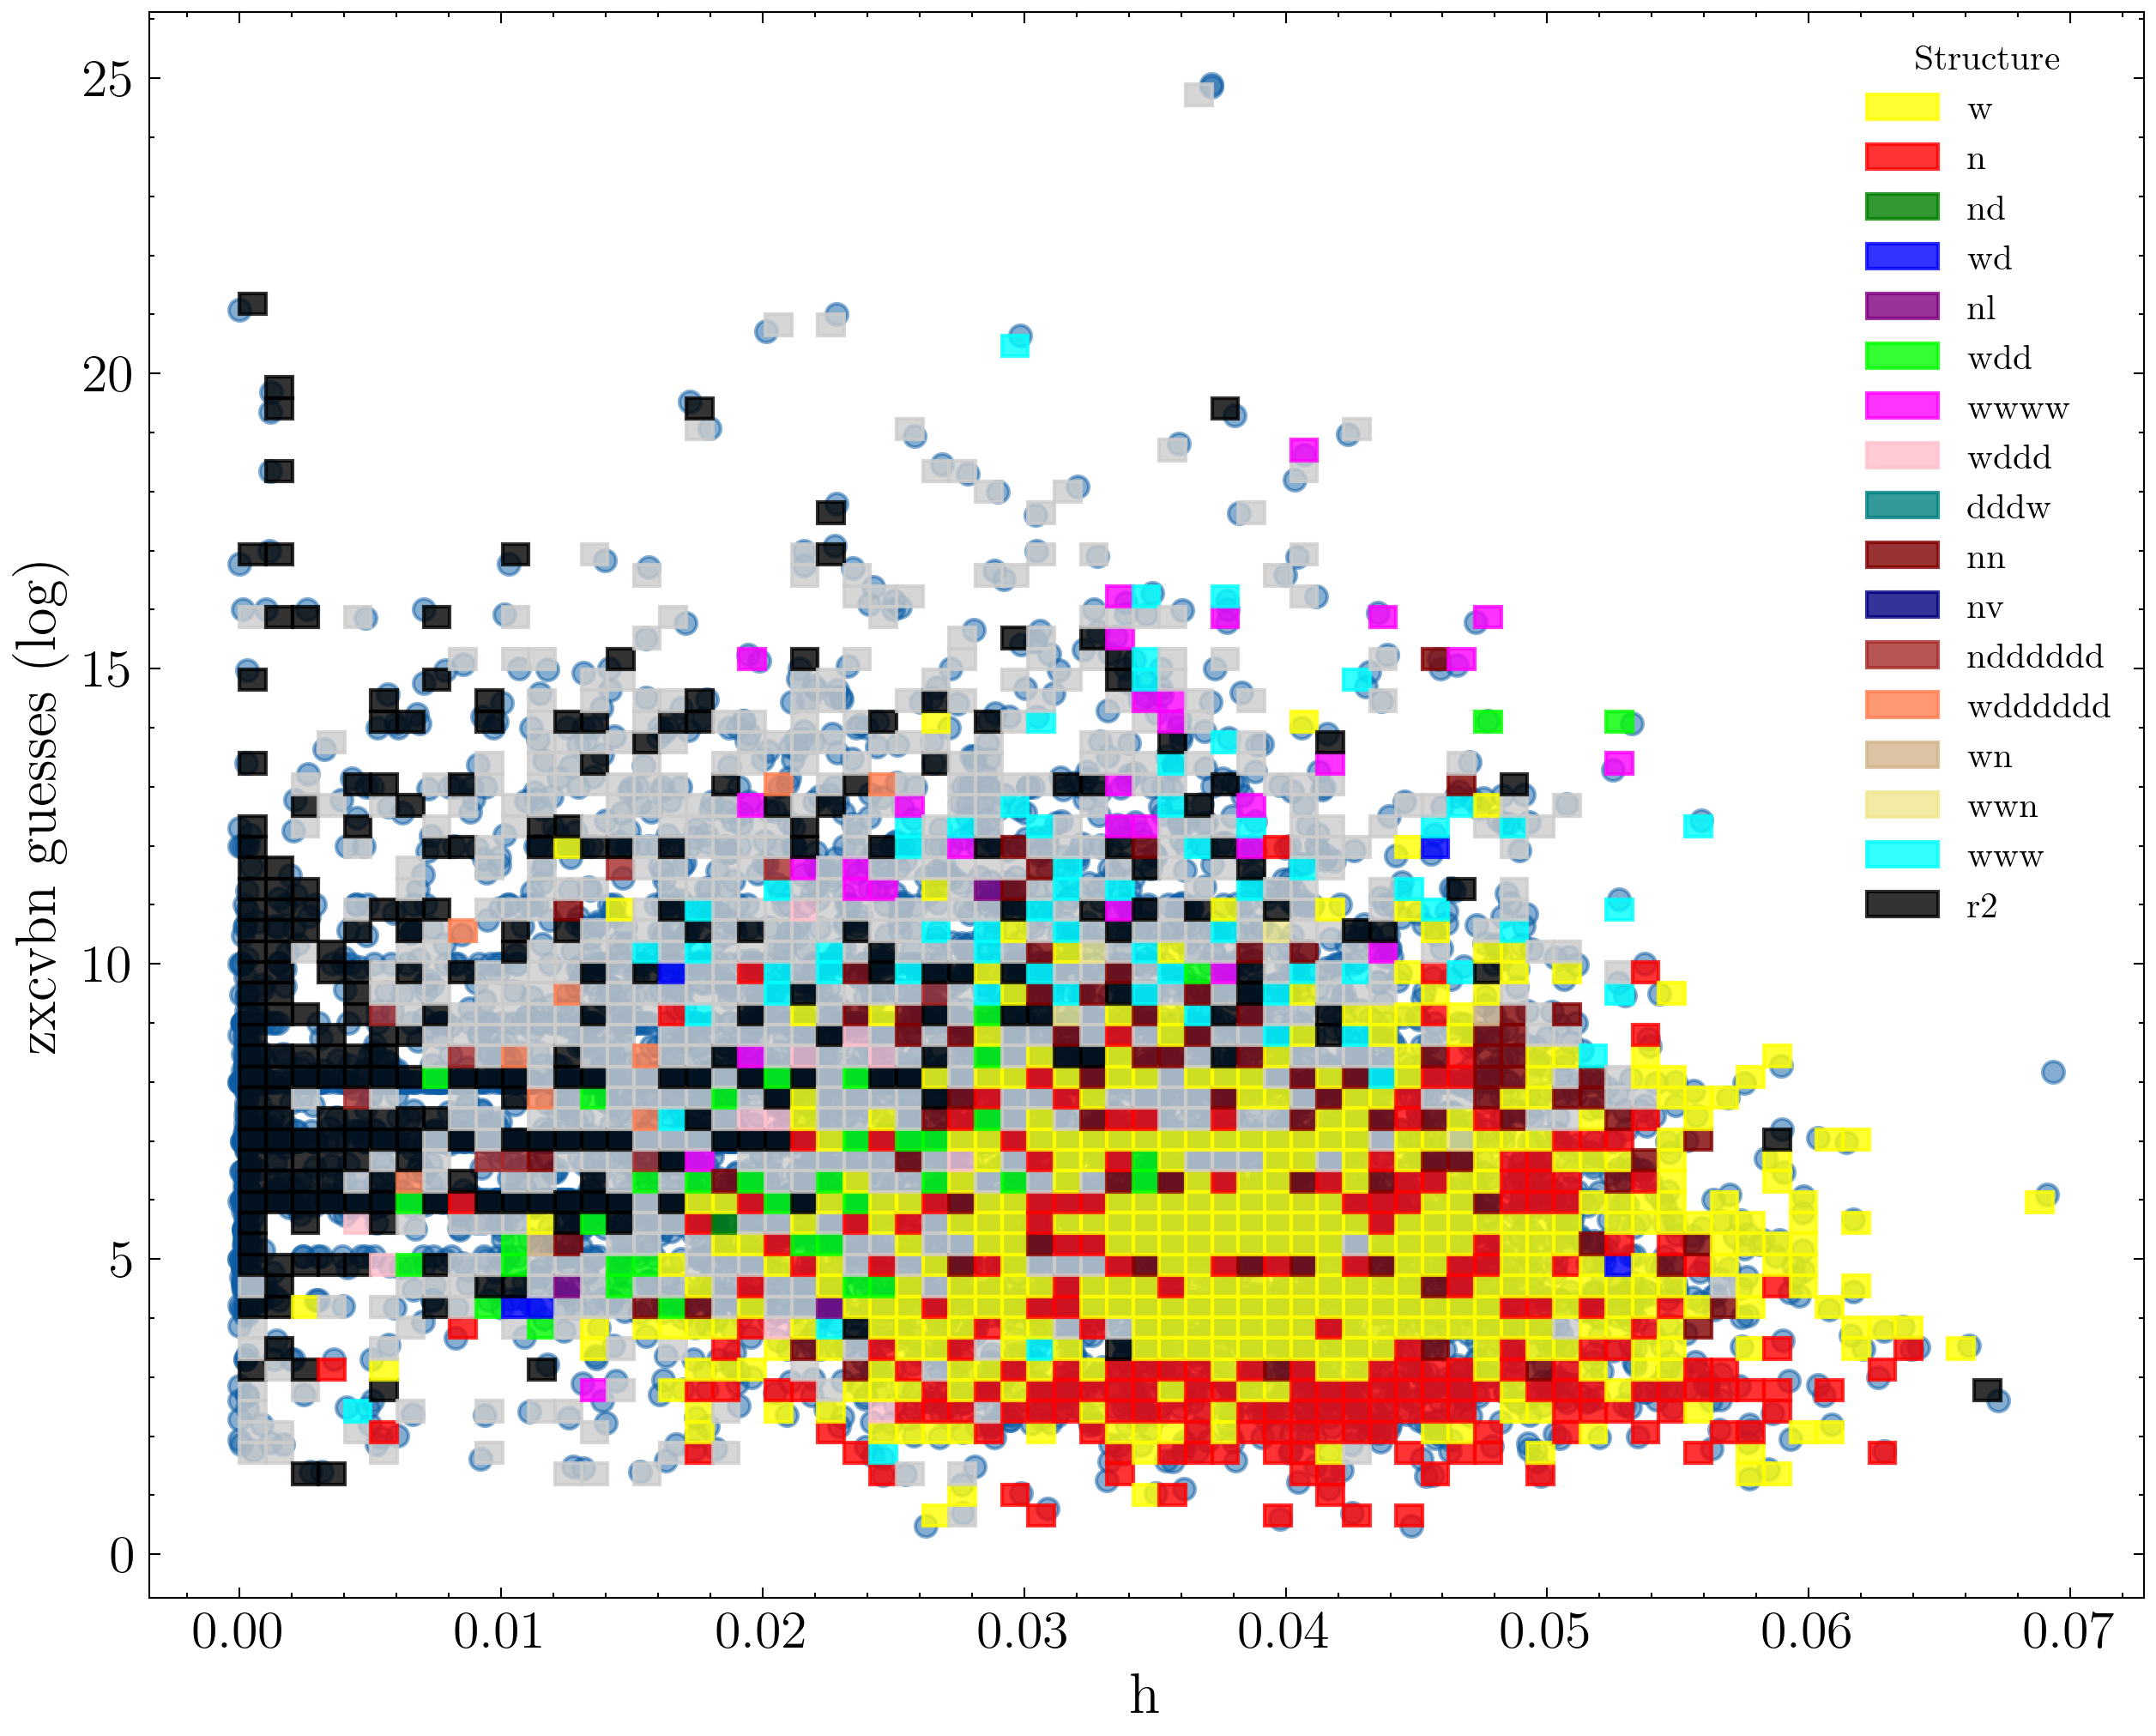
\includegraphics[scale=0.65]{figs/why_passwords/heatmap_structure.png}
        \caption{Chart showing the labelled \hmail passwords and their respective structure. Individual grids represent the most frequent structure. On the y axis we have the \zxcvbn \texttt{guesses\_log10} metric and on the x axis we have the $h$ = Markov 2-gram scores. As expected, the weakest passwords ($\bm{w}$: yellow and $\bm{n}$: red) have a high $h$ score and are predicted to be weak by \zxcvbnnocite. \srcOwnFig}
        \label{fig:heatmap_structure}
        %\vspace{-1em}
    \end{figure}

\section{Experiment: Human and LLMs as Labellers}
\label{section:experiment1}

Data labelling, particularly for password strings, is a labour intensive task. To expedite this process, we explored the effectiveness and cost-effectiveness of human versus machine labelling. We recruited freelancers from Fiverr \cite{fiverr2024} to represent the human element. On the machine side, we employed several Large Language Models (LLMs), including GPT-3.5-turbo \cite{gpt3.5}, LLaMA2-13B \cite{llama2}, and 70B, along with the Mistral-7B \cite{mistral7b}. This approach allowed us to compare the precision, efficiency, and financial implications of utilising human labour against AI technologies in the task of labelling complex datasets like passwords.

Several researchers have explored the application of Large Language Models (LLMs) for data labelling \cite{Pangakis_Wolken_Fasching_2023, Liu_2023, Møller_Dalsgaard_Pera_Aiello_2024} with positive results. Notably, this report \cite{refuelllm} cites the accuracy and significant speed up from the language models compared to human labellers.

\subsection{Freelance Labelling}
We tested the utility of freelancers from Fiverr \cite{fiverr2024} for password labelling. We took two samples of 1000 passwords from the \phpbb dataset; we selected passwords that were of length 6 and greater, $L >= 6$, and non-numeric but contained at least one digit. We hired two separate freelancers for \$50 each. The freelancers were proficient in the machine learning data labelling process but were non-native English speakers. They were selected randomly from the responses we received from a posted advert. We would categorise them as non-experts in this domain. We used Google Sheet to share the passwords and monitor the labelling progress. This method proved beneficial as we observed interesting behaviours. We took a hands on approach first by correcting the freelancers at the beginning by checking the first 50 labelled passwords. We had to do a lot of correction.

Interestingly, the second human agent enlisted additional helpers to expedite the labelling process, resulting in errors and inconsistency despite clear instructions. This was evident in the labelling document, where some labellers resorted to copying and pasting from search engine results, prioritising speed over accuracy. In contrast, the first agent focused on accuracy, seeking detailed feedback from us, but exceeded their five-day deadline and showed inconsistency in labelling. Accounting for the hands-on help, the accuracy of the extracted words was $50\% \pm 10\%$; this characteristic was the more accurate compared to chunking, deciphering the structure and tagging the passwords. Ultimately, the output from both agents proved unreliable.



\subsection{Language Models}
\paragraph{Part 1.} We started by fine-tuning the \textbf{GPT-3.5-turbo-0613} model with 825 manually labelled passwords, aiming for JSON-formatted outputs. This fine-tuning was carried out using OpenAI's Python API. The fine-tuning cost was $\sim$\$5 and was completed in a few hours. Testing involved evaluating this model against 300 passwords from the same \phpbb\ distribution, distinct from the training set. This initial fine-tuning, despite using limited data, showed success; however, 41 of the 300 (13.7\%) passwords required relabelling. The model struggled with transformations, especially elongated passwords such as \password{sssssue}, \password{6etter}, and \password{vic20oria}; the latter we assume to be \texttt{"victoria"}. Tokenisation is an important aspect of language models. We believe mislabelling could stem from tokenisation as well. Conducting further tests on the tokenisation method was beyond the scope of this chapter.

Encouraged by promising initial results, we conducted further experiments with additional open-source models. We started with smaller models, LLaMA2-13B and Mistral7B, and fine-tuned them using LoRa~\cite{Hu_Shen_et_al_2021} and QLoRa~\cite{Dettmers_Pagnoni_Holtzman_Zettlemoyer_2023} techniques. The outcomes of the initial experiment, using an 825-labelled training set and a 300-item test set from \phpbb, are presented in Figure~\ref{fig:300comp}.

\begin{figure}[t]
    \centering
    \scalebox{1}{% This file was created with tikzplotlib v0.10.1.
\begin{tikzpicture}

\definecolor{darkgray176}{RGB}{176,176,176}
\definecolor{limegreen018569}{HTML}{FF4858}
\definecolor{teal1293165}{HTML}{A1EEBD}

% \definecolor{xLightGreen}{HTML}{A1EEBD}
% \definecolor{xLightYellow}{HTML}{F6F7C4}
% \definecolor{xLightRed}{HTML}{F6D6D6}
% \definecolor{xLightBlue}{HTML}{7BD3EA}

\begin{axis}[
tick pos=both,
%title={Accuracy of the three models},
x grid style={black},
%xlabel={Model},
legend style={
    at={(0.5, -0.16)}, % Positions the legend below the x-axis
    anchor=north,      % Anchors the legend at its north side (top)
    legend columns=-1  % The number of columns the legend has, -1 for auto
},
xmin=-0.485, xmax=2.485,
xtick style={color=black},
xtick={0,1,2},
xticklabels={LLaMa2-13B,Mistral7B,GPT3.5-turbo},
y grid style={black},
ylabel={Accuracy \%},
ymin=0, ymax=100,
ytick style={color=black},
ytick={0,20,40,60,80,100},
axis lines=left, % This keeps only the left and bottom axis lines
axis line style={->}, % This adds an arrow to the end of the axes
axis y line*=left, % Specifies that the y axis line should be on the left side
axis x line*=bottom, % Specifies that the x axis line should be on the bottom side
]
\draw[draw=none,fill=teal1293165] (axis cs:-0.35,0) rectangle (axis cs:0,15.3333333333333);

\addlegendimage{ybar,ybar legend,draw=none,fill=teal1293165}
\addlegendentry{Chunks}

\draw[draw=none,fill=teal1293165] (axis cs:0.65,0) rectangle (axis cs:1,77.3333333333333);
\draw[draw=none,fill=teal1293165] (axis cs:1.65,0) rectangle (axis cs:2,89.6666666666667);
\draw[draw=none,fill=limegreen018569] (axis cs:2.77555756156289e-17,0) rectangle (axis cs:0.35,44.3333333333333);

\addlegendimage{ybar,ybar legend,draw=none,fill=limegreen018569}
\addlegendentry{Words}

\draw[draw=none,fill=limegreen018569] (axis cs:1,0) rectangle (axis cs:1.35,72.3333333333333);
\draw[draw=none,fill=limegreen018569] (axis cs:2,0) rectangle (axis cs:2.35,88.6666666666667);

\end{axis}

\end{tikzpicture}
}
    \caption{Accuracy of three models in chunking and extracting words from a password string.The models are fine-tuned using 825 passwords from the \phpbb dataset, and are tested on a separate 300 passwords from the same dataset.}
    \label{fig:300comp}
    %\vspace{-1em} 
\end{figure}
%   
\paragraph{Part 2.} In the second phase of our experiment, we augmented our training set by adding 900 passwords from the \hmail dataset. Building on the initial work with GPT-3.5 and Mistral, we expanded our test set to include 3\,062 labelled \hmail passwords. These passwords consisted primarily of characters (without digits) and were not found in dictionaries, indicating they were either phrases or obscure words. We replaced the LLaMa-13B model with a larger LLaMa2 variant, specifically using the \textit{Riiid/sheep-duck-llama-2}\footnote{\url{https://huggingface.co/Riiid/sheep-duck-llama-2-70b-v1.1}} \cite{mukherjee2023orca, platypus2023, Orca-best} model, which benefits from training on a more extensive dataset compared to the standard 70B parameter model.

\begin{figure}[t]
    \centering
    \scalebox{1}{% This file was created with tikzplotlib v0.10.1.
\begin{tikzpicture}

\definecolor{darkgray176}{RGB}{176,176,176}
\definecolor{limegreen018569}{HTML}{FF4858}
\definecolor{teal1293165}{HTML}{A1EEBD}

% \definecolor{xLightGreen}{HTML}{A1EEBD}
% \definecolor{xLightYellow}{HTML}{F6F7C4}
% \definecolor{xLightRed}{HTML}{F6D6D6}
% \definecolor{xLightBlue}{HTML}{7BD3EA}

\begin{axis}[
tick pos=both,
%title={Accuracy of the three models},
x grid style={black},
%xlabel={Model},
legend style={
    at={(0.5, -0.16)}, % Positions the legend below the x-axis
    anchor=north,      % Anchors the legend at its north side (top)
    legend columns=-1  % The number of columns the legend has, -1 for auto
},
xmin=-0.485, xmax=2.485,
xtick style={color=black},
xtick={0,1,2},
xticklabels={SheepDuck70B,Mistral7B,GPT3.5-turbo},
y grid style={black},
ylabel={Accuracy \%},
ymin=0, ymax=100,
ytick style={color=black},
ytick={0,20,40,60,80,100},
axis lines=left, % This keeps only the left and bottom axis lines
axis line style={->}, % This adds an arrow to the end of the axes
axis y line*=left, % Specifies that the y axis line should be on the left side
axis x line*=bottom, % Specifies that the x axis line should be on the bottom side
]
\draw[draw=none,fill=teal1293165] (axis cs:-0.3,0) rectangle (axis cs:-0.1,56.3030698889615);
\addlegendimage{ybar,ybar legend,draw=none,fill=teal1293165}
\addlegendentry{Chunks}

\draw[draw=none,fill=teal1293165] (axis cs:0.7,0) rectangle (axis cs:0.9,96.1463096015676);
\draw[draw=none,fill=teal1293165] (axis cs:1.7,0) rectangle (axis cs:1.9,72.8608752449379);
\draw[draw=none,fill=limegreen018569] (axis cs:-0.1,0) rectangle (axis cs:0.1,51.6982364467668);
\addlegendimage{ybar,ybar legend,draw=none,fill=limegreen018569}
\addlegendentry{Words}

\draw[draw=none,fill=limegreen018569] (axis cs:0.9,0) rectangle (axis cs:1.1,96.1789679947747);
\draw[draw=none,fill=limegreen018569] (axis cs:1.9,0) rectangle (axis cs:2.1,70.4114957544089);
\end{axis}

\end{tikzpicture}
}
    \caption{Chart showing the accuracy of three models in chunking and extracting words from a password string. The models are fine-tuned using 1\,725 manually labelled passwords from the \phpbb and \hmail dataset. Test data is 3062 passwords from the \hmail dataset.}
    \label{fig:shepduckcomp}
    %\vspace{-1em} 
\end{figure}

\subsection{Evaluation}
The models do not generalise well with different structures from ones trained on, e.g. \texttt{rosa38} and \texttt{38rosa} have the reverse grammatical structures. The labelling of the \textit{structure} were predominantly correct except for the digit counts. The models also found reversing the structure difficult. This $A \rightarrow B$ and $B \rightarrow A$ phenomena in LLM is well documented \cite{Berglund_Tong_Kaufmann_Balesni_Stickland_Korbak_Evans_2023}.

The model does not generalise well against languages. We tested the \hmail passwords that contained Spanish words with models that were trained on the \phpbb data and often the models attempted to translate words back into English.

All the models produced well structured JSON data regardless of the amount of data it was fine-tuned with.

Our initial experiment on using language models to label passwords were successful enough to warrant future research in our opinion. Further experimentation of language model is beyond the scope of this chapter and there is significant research avenues to explore. Conducting more experiments with different prompting techniques, synthetic data, more human labelled datasets, and different models can prove beneficial.

 % human v.s. machines: how to label faster
%\section{Experiment: Search Engines}
Search engines have a special function to suggest correction to the user's input. Let \( f(x) \) represent the function used by search engines to suggest corrections to user inputs, where \( x \) is the input string. This function addresses issues such as misspellings, concatenation, or low search frequency. An example is Google's \textit{"Did you mean..."} function, let this be $f_G(x)$.

Define a set of passwords \( P \) from a labeled corpus, such that \( P = \{ p_1, p_2, \ldots, p_n \} \), where each \( p_i \) satisfies the following conditions:
\begin{enumerate}
    \item \( p_i \) contains no digits.
    \item \( p_i \) is not found in any predefined dictionaries \( D \).
\end{enumerate}

Given \( |P| = 3062 \), we apply \( f_G \) to each \( p_i \), i.e. using the Google search engine: \( f_G(p_i) \) for \( i = 1, 2, \ldots, 3062 \). The outputs are saved as \texttt{HTML} files for experimental reproducibility. Finally, the results of \( f_G(p_i) \) are compared against our own labeled set \( P \).

\section{Discussion}
\label{sec::passwordninja::discussion}

In this chapter, we presented a large-scale, human-labelled password dataset, which, to the best of our knowledge, is the first of its kind. We then demonstrated its utility by using it to empirically derive new facts and insights regarding password composition and strength. Additionally, we introduced novel techniques for expediting the labelling process and demonstrated how Large Language Models (LLMs) can be employed to label passwords. The rest of this section discusses our key insights, the significance of the dataset, and the limitations of our study.

The method used to capture a dataset introduces a bias. Often, leaked datasets consist of hashes that have been cracked by various entities and subsequently redistributed. Passwords that remain uncracked are either omitted or included only in their hashed form. This omission, along with the presence of uncracked passwords, can distort the analysis. The value of the \hmail dataset lies in its acquisition through a phishing attack, allowing us to assume that it includes passwords of all complexities. In contrast, datasets derived solely from obtained hashes are likely to lack structures considered difficult to crack, such as sequences like $www$. The \hmail dataset does not exhibit signs of strict password policies, such as requirements for special characters, digits, or mixed character cases.

\subsection{Impact}
\label{sec::passwordninja::impact}

\textbf{Password Modelling:} One of the key implications of this dataset is its potential to improve password modelling. By analysing the detailed breakdown of password structures, words, tags, and transformations, researchers can develop more accurate model passwords. This can help in assessing the strength of existing password policies and identifying potential vulnerabilities in authentication systems. Moreover, the insights gained from the dataset can guide the development of new password guessing tools and techniques. Password guessing strategies are useful because they allow us to discover new vulnerabilities in our passwords and thus use that knowledge to develop better password composition policies and strength meters.

\textbf{Supervised Learning:} This labelled dataset has the potential to be used for supervised learning techniques. It can also be used for evaluation techniques of other ML techniques.

\textbf{Approximate String Matching:} Design and evaluation of new string matching algorithms. The problem of password similarity is closely related to string matching. However, measuring password similarity is more difficult than measuring normal strings. The text transformations, phonetic changes, and concatenation of other words and symbols increase the difficulty. Password similarity algorithms are important and have numerous use cases. In password strength meters, they help determine how closely a user’s password resembles existing passwords that may be deemed weak. If we are developing an algorithm to generate passwords, a similarity algorithm may be required to measure the difference between the generated password and the true password. A password similarity algorithm operates under the assumption that we have~a~model~of~the~password.

\textbf{Password Strength Meters:} The labelled dataset can serve as a benchmark for evaluating the performance of password strength meters and other tools that assess password quality. By comparing the predictions of these tools against the actual composition patterns and structures present in the dataset, researchers can identify limitations and areas for improvement in existing password strength estimation techniques.

Dictionary-based PSMs, such as the \zxcvbn PSM, rely on finding patterns in a password in order to determine the strength of the password. This means it needs to decompose the password and understand the transformations if there are any. Missed patterns could mean that a password's strength is incorrectly measured. In fact, \zxcvbn does miss some patterns as we shall in more detail below. Patterns such as \texttt{asdf1fdsa1} \cite{noauthor_password_nodate} get a high strength score of 3/4 from \zxcvbn. To answer the question, the transformations discovered in Section~\ref{sec::chp4::results} can be implemented into PSMs such as \zxcvbn to give a more accurate measure of strength.

\textbf{Synthetic Data Generation:} With the ethical issues raised against using real datasets, one can attempt to generate synthetic data that closely match real passwords. You can also create synthetic passwords based on other languages but preserving the structures.

\textbf{Natural Language Processing (NLP):} The dataset contains slang words and other transformations that can be used for natural language modelling. At least it can inform the modelling process. It can also be used for specific tasks such as Named Entity Recognition (NER) in datasets where there are spelling mistakes or accidental concatenation of words.

\textbf{Education:} By understanding common password composition patterns and the prevalence of certain structures and transformations, we can design targeted educational campaigns and materials that address specific weaknesses and promote best practices for creating strong passwords. Insights from the dataset help craft more effective risk communication strategies and guide users toward adopting more secure password habits.

\subsection{Ethical Considerations}
\label{passwordninja::ethicalconsiderations}

We have used real passwords that belong to individuals that were phished and consequently tricked into revealing their passwords. This raises few ethical issues: whether this in depth analysis will hurt those users? will it reveal any other secrets? will it identify any individuals? This dataset dates back to 2009 and therefore it is highly unlikely that the same users would have kept their passwords the same even if the identity of the individual could be revealed. Identities are highly unlikely to be revealed through our data. We have not used any PII or any other information that could link back to individuals. This dataset has also been previously used in other research papers.

This new dataset and repository of the data have been created solely for academic research purposes. The data, sourced from publicly accessible repositories like SecLists \cite{miessler_danielmiesslerseclists_2024}, does not reveal any novel information. Our analysis also does not expose any new details about the original users associated with these passwords. Importantly, this dataset is devoid of any personally identifiable information (PII).

The use of breached and leaked password datasets is well established in published research, with some studies even incorporating PII such as email addresses and dates of birth. As such, this work aligns with existing practices in the field and does not necessitate additional scrutiny. Analysing leaked datasets is crucial for advancing our understanding of how human-chosen secrets are employed, ultimately enabling us to enhance their resilience against malicious actors.

\vspace*{-0.6cm}
\subsection{Limitations}
\vspace*{-0.2cm}

There is a portion of the dataset that is labelled as R2 that could be studied further. Some of these passwords were difficult to label.
The presence of human errors and inconsistencies in the labelling process is a notable limitation of our work. It is reasonable to assume that human-labelled datasets will contain some inaccuracies. Nevertheless, these errors are generally negligible. To mitigate these issues, we propose the development of an online dashboard that allows users to continuously identify and correct any errors.

Labelling passwords in non-native languages presents additional inconsistencies for human agents, primarily due to limited vocabulary and unfamiliarity with linguistic nuances. Implementing an online portal where native speakers can rectify these errors would be advantageous over time. Such a system could also facilitate the creation of an extensive phonetic dictionary, encompassing words and names that are typically challenging to locate in centralised repositories.

A notable limitation of this study is its applicability to datasets in languages other than English or Spanish, such as Chinese. While Chinese datasets and literature are extensively researched, direct model transfer is not feasible. However, the methodology and insights into password patterns may be adaptable. Investigating how cultural differences manifest in password choices, including variations in structural patterns, vocabulary categories, and word types, could yield significant insights. Given that literature and art reflect societal and cultural contexts, passwords may similarly serve as indicators within the same domain.

Some passwords are constructed using abbreviations, codes, or acronyms that are comprehensible only to their creators. Decomposing these into meaningful components is often impractical, warranting their categorisation under the ``R2'' label. However, these passwords are typically short and susceptible to basic brute-force attacks, diminishing~the~security~of~their~cryptic~elements.

\section{Summary}
In this chapter, we present the first large-scale, human-labelled password dataset, comprising over 8\,000 passwords from the complete \hmail dataset, a selected subset of the \phpbb dataset, and machine-labelled entries from the \lizardsquad (2015) dataset. These datasets encompass a range of password complexity elements, including chunks, words, structures, tags, and transformations. The applications of this dataset are numerous, spanning supervised learning, education, and password modelling.

We have developed a rigorous model that incorporates password structure and empirical user behaviour patterns, filling a critical gap in our understanding of password security. Through analysis of real-world password datasets, we demonstrate that structure-based password policy such as three-words $(w,w,w)$ empirically and theoretically offer security advantages. However, the NCSC's previously recommended three-word password policy, while theoretically sound, fail to account for users' non-uniform word selection which follows a Zipf-like distribution. Our framework provides both theoretical foundations and practical guidelines for developing more robust authentication policies that reflect actual user behaviour rather than theoretical ideals.

We recommend extending the NCSC's password composition policy to require five words, which our models show provides comparable security to the theoretical three-word ideal even under real-world usage patterns. This recommendation maintains usability while providing demonstrably stronger protection.

Additionally, we investigated methods to streamline the time-consuming and costly process of password labelling. We employed freelancers and compared their performance with that of language models such as GPT-3.5-turbo, Mistral7B, LLaMa2, and their variations. Freelancers took approximately seven days to label \num{1000} passwords each, with results that were sometimes inconsistent. In contrast, language models proved to be~fast,~adaptable,~and~accurate.
